% \iffalse meta-comment
%
% Copyright (C) \the\year by Liu Benyuan <liubenyuan@gmail.com>
% This file may be distributed and/or modified under the
% conditions of the LaTeX Project Public License, either
% version 1.2 of this license or (at your option) any later
% version. The latest version of this license is in:
%
% http://www.latex-project.org/lppl.txt
%
% and version 1.2 or later is part of all distributions of
% LaTeX version 1999/12/01 or later.
%
% \fi
% 
% \iffalse
% <package>\NeedsTeXFormat{LaTeX2e}[1999/12/01]
% <package>\ProvidesPackage{nudtpaper}
% <package>		[2009/08/12 v1.0 By Liu Benyuan <liubenyuan@gmail.com>]
%<*driver>
\ProvidesFile{nudtpaper.dtx}[2009/08/12 v1.0 NUDT]
\documentclass[11pt]{ltxdoc}
\usepackage{nudtx}
\EnableCrossrefs
\CodelineIndex
\RecordChanges
\begin{document}
  \DocInput{\jobname.dtx}
\end{document}
%</driver>
% \fi
% 
% \def\thuthesis{\textsc{Thu}\-\textsc{Thesis}}
% \def\nudtpaper{\textsc{Nudt}\-\textsc{Paper}}
% 
% \CheckSum{1204}
% \CharacterTable
%  {Upper-case    \A\B\C\D\E\F\G\H\I\J\K\L\M\N\O\P\Q\R\S\T\U\V\W\X\Y\Z
%   Lower-case    \a\b\c\d\e\f\g\h\i\j\k\l\m\n\o\p\q\r\s\t\u\v\w\x\y\z
%   Digits        \0\1\2\3\4\5\6\7\8\9
%   Exclamation   \!     Double quote  \"     Hash (number) \#
%   Dollar        \$     Percent       \%     Ampersand     \&
%   Acute accent  \'     Left paren    \(     Right paren   \)
%   Asterisk      \*     Plus          \+     Comma         \,
%   Minus         \-     Point         \.     Solidus       \/
%   Colon         \:     Semicolon     \;     Less than     \<
%   Equals        \=     Greater than  \>     Question mark \?
%   Commercial at \@     Left bracket  \[     Backslash     \\
%   Right bracket \]     Circumflex    \^     Underscore    \_
%   Grave accent  \`     Left brace    \{     Vertical bar  \|
%   Right brace   \}     Tilde         \~}
%
% \changes{v0.99}{2009/08/12}{Initial Release}
%
% \GetFileInfo{\jobname.dtx}
% 
% \DoNotIndex{\begin,\end,\begingroup,\endgroup}
% \DoNotIndex{\ifx,\ifdim,\ifnum,\ifcase,\else,\or,\fi}
% \DoNotIndex{\let,\def,\xdef,\newcommand,\renewcommand}
% \DoNotIndex{\expandafter,\csname,\endcsname,\relax,\protect}
% \DoNotIndex{\Huge,\huge,\LARGE,\Large,\large,\normalsize}
% \DoNotIndex{\small,\footnotesize,\scriptsize,\tiny}
% \DoNotIndex{\normalfont,\bfseries,\slshape,\interlinepenalty}
% \DoNotIndex{\hfil,\par,\hskip,\vskip,\vspace,\quad}
% \DoNotIndex{\centering,\raggedright}
% \DoNotIndex{\c@secnumdepth,\@startsection,\@setfontsize}
% \DoNotIndex{\ ,\@plus,\@minus,\p@,\z@,\@m,\@M,\@ne,\m@ne}
% \DoNotIndex{\@@par,\DeclareOperation,\RequirePackage,\LoadClass}
% \DoNotIndex{\AtBeginDocument,\AtEndDocument}
%
% \IndexPrologue{\section*{索引}%
%    \addcontentsline{toc}{section}{索~~~~引}}
% \GlossaryPrologue{\section*{修改记录}%
%    \addcontentsline{toc}{section}{修改记录}}
%
% \renewcommand{\abstractname}{摘~~要}
% \renewcommand{\contentsname}{目~~录}
%
% \title{\textsc{NUDTpaper:}\,\,NUDT研究生学位论文\LaTeX{}模板使用手册\thanks{NUDT \LaTeX{} Thesis Template}}
% \author{刘本源 \\ \texttt{Liubenyuan@gmail.com}}
% \date{\fileversion\ (\filedate)}
%
% \maketitle
% \thispagestyle{empty}
%
% \begin{abstract}
% 本模板旨在提供规范的国防科学技术大学\LaTeX{}写作模板环境,
% 现支持硕士/博士学位论文格式,可以自动生成盲评、制作A3封面。
% \end{abstract}
%
% \vspace{2cm}
% \def\abstractname{免责声明}
% \begin{abstract}\noindent
% \begin{enumerate}
% \item 本模板的发布遵守 \LaTeX{} Project Public License,使用前请认真阅读协议内容
% \item 本模板创立参照官方严格的论文写作手册,并同时参照硕士/博士学位论文\textbf{doc}文档对比修改
% \item 国防科学技术大学对论文写作提供写作指南与官方\textbf{doc}模板,
% 同时提供官方的\LaTeX{}模板,本模板的出发点是方便大家使用专业的高效的论文书写工具,
% 其有点在于注重排版质量、命令规范、使用方便、更新及时,符合论文撰写说明。
% 但任何由于使用本模板而引起的论文格式审查问题均与本模板作者无关。
% \item 任何个人或组织均可以本模板为基础进行修改、扩展,生成新的专用模板,但请严格遵
% 守\LaTeX{} Project Public License 协议
% \item 欢迎提出修改意见
% \end{enumerate}
% \end{abstract}
%
% \clearpage
% \tableofcontents
%
% \clearpage
% \pagenumbering{arabic}
% \pagestyle{mainpage}
%
% \section{快速上手}
% 这部分是专门为那些想快速开始写论文的人准备的。
% \begin{description}
% \item[安装\TeX] 下载最新的\TeX{}live或者C\TeX{}并安装
% \item[字体] 用户需要具备\verb|simsun.ttf|, \verb|simhei.ttf|, \verb|simkai.ttf|,
% \verb|STZHONGS.TTF|, 上述字体都是windows自带的; 除此之外,在网上搜索(或者C\TeX{}
% 论坛)``Adobe Opentype 中文字体'',一搜一大把,确保下载下来Adobe的四款OTF字体:
% 宋,黑,仿宋,楷体。Linux用户可将上述字体复制到\verb|/usr/share/fonts/TTF|下。
% \item[试一试] 解压缩下载的模板,双击makepdf.bat(祈祷一下),如果生成了
% \verb|thesis.pdf|$\rightarrow$
% \item[那么我的那些常用的包都在么?] 你会想我的{\bf Trans}论文可以无缝
% 的复制过来么? 对于这一点,你可以修改\verb|mynudt.sty|来实现。但是{\hei 注意},大部分包
% 都在模板中了,而且{\hei 切记切记},不要擅自改动字体等版面设计,我们继续看$\rightarrow$
% \item[咦,数学公式不是很美观呀] 笔者{\hei 强烈}建议用户使用{\bf mtpro2}宏包的,怎么使用,
% 又有哪些好处,参见bookzh.sty吧!不会错的。好了,我们专注于内容本身吧$\rightarrow$
% \item[开始写了] 所有文件均采用UTF8编码,因此要保证你的\TeX{}编辑器
% (winedt, texworks, texmaker, vim, 记事本($\cdots{}$)等)支持这种编码,
% (经过一番搜索设置后)打开\verb|thesis.tex|,如果看到的是中文$\rightarrow$
% \item[漫长的写作] 手边准备着\LaTeX{}的常用帮助文档(数学,图表,引用等),
% 结合你喜欢的文献管理软件(JabRef等), 漫长的\texttt{编辑,编译,修改,编辑,
% 编译$\cdots$}过程之后,突然有一天发现你写完了$\rightarrow$
% \item[校订] 经过老师师兄师弟师妹齐心协力校正之后,你所做的只是:
% \texttt{生成明评论文,制作明评封面,生成盲评论文,制作盲评封面},
% 装订,上交$\rightarrow$
% \end{description}
% {\color{magenta} Done!}
%
% \section{模板介绍}
%
% \textsc{NUDTpaper} 旨在帮助并且推广\LaTeX{}在国防科技大学论文中的应用,
% 本文将尽可能帮助用户掌握\textsc{NUDTpaper}的安装方法,
% 如果仍旧有不清晰的地方可以参考样例文件或者
% 给作者邮件\footnote{liubenyuan@gmail.com},感兴趣的同学可以帮忙维护模板,
% 这个模板首先符合官方的设计要求,希望同学们在使用后能够提出你们的修改意见。
% 该模板很大程度上参考了6院黄老师sofoot的国防科大博士论文模板,
% 哈工大的\LaTeX{}模板以及清华的Thuthesis
% \footnote{主页:\url{http://thuthesis.sourceforge.net}},
% 有很多使用的帮助、\verb|.cls|中的命令以及版面设置均来自Thuthesis和sofoot的模板,
% 对此的引用表示感谢。
%
% {\color{blue}\fs 模板的作用在于减轻论文写作过程中格式调整的时间,
% 其前提就是遵守模板的用法,不提倡手动更改格式,不建议正文中使用
% 手动调节版面的命令,尤其禁止修改行距和使用\verb|\normalsize|,
% 否则即使使用了\textsc{NUDTpaper}也难以保证输出的论文符合学校规范。}
%
% \section{安装}
% \label{sec:install}
%
% \subsection{下载}
% \textsc{NUDTpaper} 主页:\url{http://nudtpaper.googlecode.com}。
% 模板的更新信息发布在\href{http://bbs.ctex.org}{Ctex论坛}。
% \nudtpaper{}的开发版本同样可以在\textsc{gitorious}上获得。
%
% \subsection{模板的组成部分}
% 下表列出了 \nudtpaper{} 的主要文件及其功能介绍,学习模板的最好办法
% 就是参考thesis.pdf!
% \begin{center}
% \begin{longtable}{l|p{8cm}}
% \toprule
% {\hei 文件(夹)} & {\hei 功能描述}\\\midrule
% \endfirsthead
% \toprule
% {\hei 文件(夹)} & {\hei 功能描述}\\\midrule
% \endhead
% \endfoot
% \endlastfoot
% nudtpaper.ins & 模板驱动文件 \\
% nudtpaper.dtx & 模板文档代码的混合文件\\
% nudtpaper.cls & 模板类文件\\
% nudtpaper.cfg & 模板配置文件\\
% thesis.bib & 参考文献样式文件\\
% \hline
% mynudt.sty & 在这里添加你自己的宏包 \\
% thesis.tex & 示例文档主文件\\
% ref/ & 示例文档参考文献目录\\
% data/ & 示例文档章节具体内容\\
% figures/ & 示例文档图片路径\\
% \textbf{nudtpaper.pdf} & 用户手册(本文档)\\
% \textbf{thesis.pdf} & 示例文档 \\
% \bottomrule
% \end{longtable}
% \end{center}
%
% \subsection{\TeX{}系统的选择}
% 有网络环境的用户推荐安装\href{http://www.tug.org/texlive}{\TeX{}live},
% \href{http://miktex.org}{MiKTeX}或者\href{http://www.ctex.org}{C\TeX},
% 对于无网络环境的,主要是针对教研室用户,推荐{\TeX{}live}或者C\TeX{}完整版,安装
% 过程很简单,一路下一步即可,但是需要\textbf{注意:}
%
% \begin{description}
% \item[字体] TTF选项默认调用Windows系统字体,其中楷体、仿宋需要安装Office;OTF选项需要
% Adobe的商业字体(可以使你的论文更加漂亮!),这些中文字体(宋,黑,仿宋,楷体)可以从
% \href{http://dl.getdropbox.com/u/857066/adobe_chinese_otf.7z}{这里下载},
% 如果上述链接不能使用,请搜索\textsc{Adobe Opentype 中文字体}自行下载。
% 英文字体使用Windows自带。起始更推荐几款Times(Arial)类似的OTF英文字体,可以使用
% 更多排版、段落的字体特性。
% \item[粗宋] 模板中在需要宋体加黑的地方需要使用\textbf{华文中宋}, 即STZHONGS.TTF。
% \item[xeCJK] 无网络环境中,C\TeX{}完整版和\TeX{}live最新版都包括了需要的xeCJK版本。
% \end{description}
%
% \subsection{使用模板}
% \label{sec:install-cls}
% {\hei 注:默认的发行版本已经包含了可以使用的模板环境,
% 包括编译好的cls以及论文样例源文件,
% 想快速上手的话,可以直接参看\verb|thesis.tex|,进行修改。
% 写作的过程就是将你的论文的内容放到\verb|data|文件夹中,
% 图片放到\verb|figures|文件夹中,用\textsc{jabref}修改\verb|thesis.bib|即可。}
%
% 当用户需要编译生成自己的PDF版论文时,需要依次输入:(注意了,如果不是使用nomencl,
% 则无需使用第二个命令)
% \begin{shell}
% $ xelatex thesis
% $ # makeindex -s nomencl.ist -o thesis.nls thesis.nlo
% $ bibtex thesis
% $ bibtex thesis
% $ xelatex thesis
% $ xelatex thesis
% \end{shell}
%
% 而为了简化用户使用,模板中提供了快捷脚本文件:
% \begin{shell}
% # 下面命令可以直接生成thesis.pdf,你可能只需要这步
% C:\> makepdf.bat
% # linux用户可以直接使用makefile
% $ make pdf
% \end{shell}
% 现在,就要进入激动人心的写作过程了。
%
% \section{使用说明}
% \label{sec:how-to-use}
% 首先,一篇论文(电子信息工程专业为例),主要的构成就是
% 封面导言,正文,表格,图片,公式,
% 交叉引用及文献索引这五部分,下面将分别详细讲解。
%
% \label{sec:howtoask}
% 在开始之前,先问自己几个问题:
% \begin{compactenum}
% \item 我是不是已经掌握了 \LaTeX{} 基础知识?
% \item 我是不是认真地阅读了模板文档?
% \item 周围有没有同学可以帮我?
% \end{compactenum}
% 更推荐用户去阅读示例文档的源代码,改写会给你一个快速的开始。
%
% \subsection{示例文件}
% \label{sec:example}
% 该示例文件是顶层的文件,包括论文属性设置、章节的安排、参考文献附录等。
% 细节用户可以参考\verb|thesis.tex|和\verb|data/|文件夹。
%
% \subsubsection{模板选项}
%
% 论文的第一句话是调用模板:
% \changes{v2.0}{2010/11/10}{增加盲评的说明}
%
%    \begin{macrocode}
%<thesis>%1. 规范硕士导言
%<thesis>% \documentclass[master,ttf]{nudtpaper}
%<thesis>%2. 规范博士导言
%<thesis>% \documentclass[doctor,twoside,ttf]{nudtpaper}
%<thesis>%3. 如果使用是Vista
%<thesis>% \documentclass[master,ttf,vista]{nudtpaper}
%<thesis>%4. 建议使用OTF字体获得较好的页面显示效果
%<thesis>%   OTF字体从网上获得,各个系统名称统一,不用加vista选项
%<thesis>%   如果你下载的是最新的(1201)OTF英文字体,建议修改nudtpaper.cls,使用
%<thesis>%   Times New Roman PS Std
%<thesis>% \documentclass[doctor,twoside,otf]{nudtpaper}
%<thesis>%5. 如果想生成盲评,传递anon即可,仍需修改个人成果部分
%<thesis>% \documentclass[master,otf,anon]{nudtpaper}
%<thesis>%
%    \end{macrocode}
%    \begin{macrocode}
%<*thesis>
\documentclass[master,otf]{nudtpaper}
\usepackage{mynudt}

%</thesis>
%    \end{macrocode}
%
% 模板的参数设置(开关)描述见:
%
%\begin{description}
%\item[master,doctor]
% 硕士论文用master,博士论文就用doctor
%\item[twoside]
% 指定论文为单面打印还是双面打印,当使用\verb|twoside|选项之后,
% 论文会将章节开在奇数页右手边,默认为\verb|openany|单面打印。
%\item[ttf,otf]
% 决定使用何种字体,TTF默认使用Windows自带的字体,而OTF则使用Adobe的字体(需要下载),
% TTF字体的优势是满足学校论文对于字体的要求,缺点是制作出来的PDF文件在浏览时可能发虚,
% 而OTF字体屏幕显示饱满,而且字体有很多选项可以方便\XeTeX{}排版。推荐使用\textbf{otf}
% 选项。不论何种选项,都需要安装宋体中宋(STZHONGSONG)字体(Windows自带)。
%\item[vista]
% 使用\textsc{vista}的用户当调用模板的TTF字体时,系统默认的楷体、仿宋名称是KaiTi和FangSong,
% 而不是KaiTi\_GB2312,这里加入开关进行切换。
%\item[anon]
% 是否为盲评版本,如需盲评,请加上anon。
%\end{description}
%
% 如果需要使用自己定义的命令、宏包,请放于\verb|mynudt.sty|中。
% 事实上,该文件中已经添加了很多有用的宏包和命令,你可以参照修改。
% 这些之所以没有放到模板中,一则为了简洁,二则赋予用户在格式之外更多的自由。
% 里面的宏包有:代码高亮、算法环境、向量命令等,请仔细查看。
%
% 样例文件默认的是硕士论文(master),OTF字体(otf)。
%
% \subsubsection{封面导言}
% 官方模板中设计论文题目、作者等信息可以跟填空一样完成:
%
% \begin{description}
% \item[论文封头]
% 主要有四部分内容,中图分类号,学号,论文密级和UDC。
% 密级分为:\textbf{秘密} 或者 \textbf{公开}。
%    \begin{macrocode}
%<*thesis>
\classification{TP957}
\serialno{0123456}
\confidentiality{公开}
\UDC{}
%</thesis>
%    \end{macrocode}
%
% \item[论文题目,作者,日期]
% 分别包括中文和英文两部分,由于论文题目可能超过1行,
% 我们提供额外的一个命令\verb|\displaytitle|用来在
% 授权书中填入(限定为)单行的题目; 中文日期需要中文输入大写,英文日期为月年,
% 在论文最终完成后,请\textbf{手动}设定日期。
%
%    \begin{macrocode}
%<*thesis>
\title{国防科大学位论文\LaTeX{}模板\\
使用手册}
\displaytitle{国防科学技术大学学位论文\LaTeX{}模板}
\author{张三}
\zhdate{\zhtoday}
\entitle{How to Use the \LaTeX{} Document Class for NUDT Dissertations}
\enauthor{Zhang San}
\endate{\entoday}
%</thesis>
%    \end{macrocode}
%
% \item[论文分类及其他]
% 主要是作者的学科类别,研究方向,导师信息等。
% 每一项都包括中英文信息:
%
%    \begin{macrocode}
%<*thesis>
\subject{通信与信息工程}
\ensubject{Information and Communication Engineering}
\researchfield{自动目标识别与模糊工程}
\supervisor{李四\quad{}教授}
\cosupervisor{王五\quad{}副教授} % 没有就空着
\ensupervisor{Professor Li Si}
\encosupervisor{}
\papertype{工学}
\enpapertype{Engineering}
%</thesis>
%    \end{macrocode}
%
% \item[中英文摘要]
% 论文中需要写中文以及英文摘要,页码为小写罗马字母,关键字为黑体,
% 英文关键字为\verb|Arial|,
% 模板中定义了相关环境\verb|\cabstract|以及\verb|\eabstract|来书写摘要,
% 以及\verb|\ckeywords|以及\verb|\ekeywords|来写关键字。
% 建议用户将摘要单独放在在\verb|abstract.tex|文件中,
% 在正文中\verb|\begin{cabstract}
国防科学技术大学是一所直属中央军委的综合性大学。1984年,学校经国务院、中央军委和教育部批准首批成立研究生院,%
肩负着为全军培养高级科学和工程技术人才与指挥人才,培训高级领导干部,从事先进武器装备和国防关键技术研究的重要任务。%
国防科技大学是全国重点大学,也是全国首批进入国家“211工程” 建设并获中央专项经费支持的全国重点院校之一。%
学校前身是1953年创建于哈尔滨的中国人民解放军军事工程学院,简称“哈军工”。
\end{cabstract}
\ckeywords{国防科学技术大学; 211; 哈军工}

\begin{eabstract}
National University of Defense Technology is a comprehensive national key university based in Changsha, %
Hunan Province, China. It is under the dual supervision of the Ministry of National Defense %
and the Ministry of Education, designated for Project 211 and Project 985, %
the two national plans for facilitating the development of Chinese higher education. %

NUDT was originally founded in 1953 as the Military Academy of Engineering in Harbin of Heilongjiang Province. %
In 1970 the Academy of Engineering moved southwards to Changsha and was renamed Changsha Institute of Technology.%
 The Institute changed its name to National University of Defense Technology in 1978.

\end{eabstract}
\ekeywords{NUDT; MND; ME}

|即可。其格式为:
%
% \begin{example}
% \begin{cabstract}
% 中文摘要
% \end{cabstract}
% \ckeywords{关键字}
%
% \begin{eabstract}
% Abstract
% \end{eabstract}
% \ekeywords{Key}
% \end{example}
% \end{description}
%
% \subsubsection{框架构成}
%
% 在定义完论文元素之后,就可以开始写论文正文了。用\LaTeX{}写论文的文件目录构成
% 可以很随意,模板中将图形文件单独放到一个目录中\verb|figure|中,论文正文各个
% 章节置于\verb|data|中;当然也以以\verb|chapter|为目录。
%\changes{v2.2}{2011/05/27}{使用nomencl包管理符号列表}
%\changes{v2.2}{2011/07/08}{默认使用nomencl管理参考文献}
%\changes{v2.2}{2011/09/10}{回复原先使用的denotation方式添加符号列表}
% 
% 如果使用nomencl制作符号列表,在文档开始前要加入\verb|\makenomenclature|命令
% 默认还是使用denotation的方式。nomencl可以参考第二章相关章节,而denote方式
% 请参考\verb|data/denotation.tex|文件(简单的列表环境)。
% 
%<thesis>% 加入makenomenclature命令可用nomencl制作符号列表。
%
%    \begin{macrocode}
%<*thesis> 

\begin{document}
\graphicspath{{figures/}}
%</thesis>
%    \end{macrocode}
% 制作完封面后就是正文四大部分了,分别为:
%
% \begin{compactenum}
% \item frontmatter: 生成目录,图目录,表目录
% \item midmatter: 摘要,符号列表
% \item mainmatter: 正文,致谢,文献,成果
% \item backmatter: 附录
% \end{compactenum}
%
%<thesis>% 制作封面,生成目录,插入摘要,插入符号列表 \\
%<thesis>% 默认符号列表使用denotation.tex,如果要使用nomencl \\
%<thesis>% 需要注释掉denotation,并取消下面两个命令的注释。 \\
%<thesis>% cleardoublepage% \\
%<thesis>% printnomenclature% \\
%
%    \begin{macrocode}
%<*thesis>
\maketitle
\frontmatter
\tableofcontents
\listoftables
\listoffigures

\midmatter
\begin{cabstract}
国防科学技术大学是一所直属中央军委的综合性大学。1984年,学校经国务院、中央军委和教育部批准首批成立研究生院,%
肩负着为全军培养高级科学和工程技术人才与指挥人才,培训高级领导干部,从事先进武器装备和国防关键技术研究的重要任务。%
国防科技大学是全国重点大学,也是全国首批进入国家“211工程” 建设并获中央专项经费支持的全国重点院校之一。%
学校前身是1953年创建于哈尔滨的中国人民解放军军事工程学院,简称“哈军工”。
\end{cabstract}
\ckeywords{国防科学技术大学; 211; 哈军工}

\begin{eabstract}
National University of Defense Technology is a comprehensive national key university based in Changsha, %
Hunan Province, China. It is under the dual supervision of the Ministry of National Defense %
and the Ministry of Education, designated for Project 211 and Project 985, %
the two national plans for facilitating the development of Chinese higher education. %

NUDT was originally founded in 1953 as the Military Academy of Engineering in Harbin of Heilongjiang Province. %
In 1970 the Academy of Engineering moved southwards to Changsha and was renamed Changsha Institute of Technology.%
 The Institute changed its name to National University of Defense Technology in 1978.

\end{eabstract}
\ekeywords{NUDT; MND; ME}


\begin{denotation}

\item[HPC] 高性能计算 (High Performance Computing)
\item[cluster] 集群
\item[Itanium] 安腾
\item[SMP] 对称多处理
\item[API] 应用程序编程接口
\item[PI]	聚酰亚胺
\item[MPI]	聚酰亚胺模型化合物,N-苯基邻苯酰亚胺
\item[PBI]	聚苯并咪唑
\item[MPBI]	聚苯并咪唑模型化合物,N-苯基苯并咪唑
\item[PY]	聚吡咙
\item[PMDA-BDA]	均苯四酸二酐与联苯四胺合成的聚吡咙薄膜
\item[$\Delta G$]  	活化自由能~(Activation Free Energy)
\item [$\chi$] 传输系数~(Transmission Coefficient)
\item[$E$] 能量
\item[$m$] 质量
\item[$c$] 光速
\item[$P$] 概率
\item[$T$] 时间
\item[$v$] 速度

\end{denotation}


%</thesis>
%    \end{macrocode}
%
%<thesis>%书写正文,可以根据需要增添章节; 正文还包括致谢,参考文献与成果
%\changes{v1.4}{2009/10/31}{将成果移动到参考文献之后}
%
%    \begin{macrocode}
%<*thesis>
\mainmatter
\chapter{绪论}

\section{课题研究背景}

\subsection{计算机硬件系统的并行化与异构化趋势}
计算机行业从它诞生伊始就保持着日新月异的发展势头。摩尔定律(Moore's Law)FIXME:citehere的神奇预言
在过去的半个世纪中准确地反映了半导体与集成电路工业的发展速度:
集成电路上的晶体管数量每18个月翻一番。在摩尔定律的作用下,单个微处理器(microprocessor)的时钟频率
越来越高,处理器性能也随之不断提高。早期计算机均采用单一微处理器作为计算部件,其性能的提高主要依赖
微处理器运算速度的提高。但随着计算机行业持续快速的发展,仅仅提高单个处理器的运算速度已经不足以使
整个计算机系同的性能得到明显提升。

首先,单个处理器的性能提高有其极限,由于功耗问题FIXME:citehere以及晶体管器件本身物理特性的限制,
单个微处理器的频率不可能无限提高;其次,随着计算机系统结构日益复杂和多样化,
访存延迟、存储器带宽等因素可能成为制约性能的主要瓶颈;此外,程序中可发掘的指令级
并行(ILP)能力有限,单一指令流已经难以充分利用高速处理器的处理能力。
因此,当今业界主流厂商已经将眼光投向并行硬件,包括多处理器(multi-processor)计算机、
多核处理器(multi-core processor)以及面向特定应用的协处理器(coprocessor),
希望通过为用户提供多个处理器或为特定应用需求提供专用处理器来获得更高的性能。

2001年IBM推出了首款通用双核(dual-core)处理器,此后,各大主流厂商相继推了不同系列的多核处理器,单个
处理器包括的核心数目不等,有的处理器核心数目可以达到16或者更多(如AMD Opteron系列,Intel Xeon系列等)。
短短几年之内,多核处理器已经占据市场主流位置,从超级计算机到高性能服务器,从桌面PC到移动通信设备,
多核处理器在许多领域都得到了广泛应用。

协处理器一般是针对特定应用而设计的处理器,如浮点计算、图形处理、信号处理、加密解密等。相较于通用
处理器,协处理器可能缺乏某些功能,但在特定的功能上具备突出的性能优势。许多计算机系统都配备一个或
多个协处理器,用以辅助CPU执行计算。图形处理器(Graphics Processor Unit, GPU)是当前应用最为广泛的一类协处理器,
它最开始被专门设计于图形处理问题,协助CPU完成图形渲染等工作,但近几年GPU已经越来越成为一种“通用”计算设备,
主流GPU厂商已经为在GPU上执行通用计算提供支持软硬件支持采取了许多努力。
GPU采用流处理(stream processing)编程模型,这是一种类似于SIMD(Single Instruction Multiple Data)
的编程模型FIXME:citehere。在流处理模型中,一组数据中的每一个单元都被
施加同一操作,一般将这种操作称之为Kernel。Kernel可以是一段程序,允许有一定的程序逻辑,而不限于单一指令,
这比SIMD提供了更高的灵活性。在硬件设计上,GPU通常拥有数百甚至上千个核心,Kernel被流水化执行,这可以大大加速
数据级并行问题的执行速度。

随着多核处理器与面向特定问题的协处理器的兴起,由通用处理器与协处理器组成异构硬件系统
(heterogeneous architecture)也已经成为当前计算机系统的主流构成模式。
由国防科学技术大学研制,在2013年度Top500FIXME:citehere评比中
排名第一的天河二号超级计算机,就采用了这种异构系统设计:它的每个计算结点由两颗Xeon E5 12核处理器(CPU)
与三颗Xeon Phi 61核协处理器(GPU)组成,CPU+GPU的硬件配置为大规模科学计算提供了强大的驱动力。在桌面
计算机市场上,一般的PC机都配备了专门的图形处理器,这些现代图形处理器,除协助CPU完成
图形渲染方面的任务之外,也支持通用计算,允许PC机用户在显卡上进行通用计算编程。
最新的智能手机也已经开始采用GPU来辅助CPU执行计算,以期为游戏应用提供更强的计算支持。

在更加宏观的层次上,并行硬件一直是提供大规模计算能力的主要技术。互联网上存在着大量的服务器集群,由数十台甚至
上百台独立计算机通过通用网络互联,搭建成的集群系统为大规模事务处理提供了强力支持。由成百上千个高性能
计算结点通过专用网络互联组成的超级计算级,使大规模科学计算问题顺利执行。这些宏观计算机系统由独立的计算机结点
组成,每个结点独立并行地执行任务,每个结点又是由并行处理器、协处理器等并行硬件构成的异构系统。

总之,并行化与异构化是当今计算机硬件系统的主流发展趋势,在可以预见的将来,计算机性能的提高将以并行硬件
的驱动与异构硬件的利用为主要手段。

\subsection{并行化与异构化硬件的软件支持}
多核处理器与协处理器为设计实现更高性能的计算机系统提供了硬件支持,如何适应
硬件的发展,有效地利用这些硬件资源,为程序员提供易用的、高效的编程工具,是提高并行硬件应用能力
的关键问题。并行编程工具的设计需要兼顾两个核心特性:FIXME:emphasizehere高效性与易用性。
高效性是指并行编程工具必须能够充分开发并行硬件的计算能力,最大程度地利用硬件资源;
易用性是指在有效开发硬件并行能力的前提下,编程工具应该是易用的,并行程序设计的难度与复杂度不能过高。
当前已经有多种并行编程工具得到了广泛使用,这些工具有的
针对多核处理器设计,有的针对异构硬件设计,有的适用于数据并行问题,有的适用于任务并行问题。
这些广泛应用的并行编程技术包括多线程、消息传递接口、并行程序语言、编译器制导指令等,
它们特点各异,在通用性、适用问题方面都有不同,下面分别简要介绍。

多线程(multithreading)技术是在传统串行编程技术的基础上发展起来一种编程模型,
它的出现早于多核处理器。一个线程在逻辑上是一个独立指令流,不同线程的指令流可以在单一处理器上交替
执行以隐藏一些耗时较高的操作(如IO),避免处理器空转,提高处理器的吞吐率。
在多核处理器上,多个线程可以真正“并行”地执行。使用多线程编程模型,编程者显式地
将整个任务划分为独立的子任务,不同的子任务在不同的线程中执行,从而利用更多处理器资源,
缩短整个程序的运行时间。多线程支持通常由操作系统(Operating System)提供,是一种非常成熟的并行
编程技术,POSIXFIXME:citehere线程是多线程模型的POSIX标准,Pthreads在多种操作系统上均有实现。

消息传递接口(Message Passing Interface, MPIFIXME:citehere)是一套并行程序库接口规范,
它以多线程技术为基础,定义了线程间
通信的标准方法,最初定位用于分布式内存计算机系统,但也适用于其他体系结构的计算机系统。MPI定义的标准
通信接口功能全面,问题描述能力强大,具被性能高、可扩展性强、可移植性强的特点,长期以来一直都是高
性能计算领域的主要编程模型。

多线程技术与MPI技术都是在已有的串行程序语言之上,通过构建程序库的方式为并行编程提供支持。这种方式的
好处是硬件控制能力强,执行效率高,缺点是受限于已有的编程语言特性,细节隐藏能力差,编程复杂度高。
并行程序语言采用一种不同的思路,从语言层面为并行程序提供支持。并行程序语言一般通过提供特殊的并行语法
结构来表达程序中的并行部分,但在底层实现仍采用传统的多线程与MPI技术,任务并行化的工作由编译器自动完成。
并行编程语言的抽象层次一般较高,更加注重语言的易用性,对编程者隐藏并行硬件细节。并行程序语言一直
是并行软件技术的研究热点,这部分内容将在下一章着重介绍。

编译器制导指令(Compiler Directive)是一种介于并行程序库与并行程序语言之间的并行编程技术,
它允许程序员在源代码中插入专用的制导指令(directive)来指出
程序中的并行部分,并在必要之处加入同步互斥及通信。编译器识别这些制导指令,对程序做自动并行化处理。
编译器也可以视情况忽略这些制导指令,这时程序退化为串行程序。这种技术只需要程序员做简单的制导工作,
具有较好的可移植性,可以根据硬件资源的数量自动调整并行度,缺点在于难以调试,缺乏错误处理,对线程
粒度控制较弱,同时很难应用于非共享内存计算机系统。编译器制导指令技术的代表是OpenMPFIXME:citehere。

开发协处理器并行能力的技术在学术界与工业界都受到高度关注,发展也十分迅速。Nvidia公司针对自己的GPU
首先提出了CUDA编程架构,使用CUDA C语言对GPU进行编程,CUDA C是一种C语言的扩展语言FIXME:citehere。
CUDA C在一定程度上暴露了GPU的硬件细节,用户对程序行为的控制力强,程序性能较高。著名的
非盈利技术联盟Khronos Group针对异构计算提出了OpenCL标准FIXME:citehere,Nvidia与AMD公司分别在自己的GPU上支持OpenCL
实现。编译器制导指令技术在协处理器上也得到了应用,代表有OpenACC与OpenHMPP。FIXME:citehere

总体上,并行程序设计的难度远远高于串行程序设计。在基于传统串行程序语言的解决方案中,编程者不仅需要
关注于解决问题的程序逻辑,还需要显式地处理各种并行细节,诸如线程创建、内存管理、消息传递、任务划分等。
并行程序语言从根本上解决了编程难的问题,但现有的实现技术效果仍不理想,多数研究成果只能适用于
特定领域特定问题,通用性有限。相较于并行硬件的发展,并行软件技术的发展处于相对滞后的状态,现阶段
并行软件技术还没有一个完美的解决方案。高效性与易用性的平衡与兼顾仍然是一个亟待解决的关键问题。

\section{课题研究意义}
正如上一小节所说,计算机硬件系统结构的主流发展趋势是并行化与异构化,而开发并行化与异构化硬件的计算能力
需要相应的并行编程技术提供编程工具。未来计算机系统的性能提高,关键就在于如何从软硬件两方面开发计算机系统
的并行执行能力。这其中,并行编程工具既要适应硬件的特性以提高执行效率,又要独立于不同的硬件结构提供易用
的编程界面,高效性是基本要求,在保证高效性的前提下尽量兼顾易用性。

具体来说,软件工具需要解决的问题有下列三点,其中前两点是实现并行软件的高效性要求,第三点是易用性要求。
\begin{itemize}
  \item 如何最大限度地开发并行硬件(包括多核通用处理器与众核协处理器。)的计算能力?
  \item 如何设计编程模型,使异构系统中通用处理器与协处理器更加有效地协调配合?
  \item 如何对用户隐藏计算机系统的并行硬件细节,降低并行程序设计的难度?
\end{itemize}

本论文着眼于上述并行软件需要解决的三个问题,对并行程序语言展开研究,
设计了一门数据并行程序语言Rat,为编程者提供一个抽象层次高、表达能力强、细节隐藏好的编程界面,大大降低
并行程序设计的难度。并行程序语言从根本上解决并行编程难的问题,对降低并行计算机系统上的应用开发难度、
提高并行计算机可用性具有重要意义。

为了保证高效性,Rat语言的设计充分考虑了GPU的硬件特点,Rat语言编译得到的程序可以在GPU上高效执行。同时,
借鉴函数式程序语言的优良性质,提出一种驱动同异构硬件协同工作的有效方法,能够发掘独立于问题的
程序并行性。这对于利用未来计算机异构硬件系统也也具有重要意义。

采用Rat语言编写的并行程序运行在一个运行时系统之上,该运行时系统可以根据不同的硬件配置采用不同的
运行时策略,这样既保证了对硬件的充分利用,由保证了较强的可移植性,使Rat程序在不同硬件配置下均可
达到比较理想的性能。

\section{主要研究内容}
函数式并行程序语言Rat的研究内容主要分为两方面:前端语法设计与后端编译实现技术。其中前端语法设计着重实现
并行编程工具的易用性,后端编译实现技术着重实现并行编程工具的高效性。

\subsection{并行程序语言语法设计}
Rat语言的语法设计旨在为编程者提供一个通用、易用的并行编程模型,Rat语言具备以下优良特性:
\begin{itemize}
  \item 抽象层次高。编程者在编程解决问题时只需要关注问题本身的逻辑,无需关注底层的并行实现细节,线程管理、
    内存管理、任务划分等工作由编译器与运行时系统维护。
  \item 表达能力强。Rat精心选取了一组并行原语,使用这一组有限的并行原语就可以方便地描述一大类数据并行问题。
  \item 语法简洁精巧,易学易用。
\end{itemize}

\subsection{并行程序语言编译实现技术}
Rat语言的设计目标是兼顾易用性与高效性。易用性由它的语法设计提供,高效性则有赖于它的编译实现技术。
本论文在Rat语言的编译实现技术方面主要包括下列研究点:
\begin{itemize}
  \item 并行虚拟机的设计。并行虚拟机是对并行硬件的抽象,它运行精简的指令集,易于分析和优化,并且在
    并行硬件上有高效实现。
  \item 开发协处理器的并行计算能力。Rat的首个实现采用Nvidia公司的GPU作为并行计算硬件,作为并行虚拟机
    的实现平台。在编译实现过程中着重考虑如何充分利用GPU的流处理器资源、共享存储器资源,
    如何达到更高的访存带宽等,采取了一些优化技术。
  \item 开发异构硬件的系统工作能力。借鉴函数式程序语言的优良特性,对如何驱动CPU与GPU协同、并行工作展开研究,
    提出一种与具体问题无关的并行性发掘技术,使不同的处理器资源发挥各自所长,提高系统整体的性能。
\end{itemize}

\section{论文结构组织}
本论文设计并实现了一门并行程序语言Rat。全文组织结构如下:

第一章介绍了论文的研究背景,指出计算机硬件并行化与异构化的发展趋势,概括了并行软件技术的发展目标,
阐述了本课题的研究意义,简述了本课题的主要研究内容。

第二章介绍了并行软件技术领域的国内外研究现状,分析现有研究采用的方法,取得的成果以及存在的不足。

第三章详细说明了Rat语言的语法设计,分别就函数式语言特性、类型系统、向量原语展开描述。

第四章说明Rat语言编译实现所采用的关键技术,包括并行虚拟机的设计、并行虚拟机在并行硬件上
的实现与优化、异构硬件系统的协同工作技术研究与并行自动化技术研究等方面。

第五章FIXME:shiyan

第六章对论文的工作进行总结,指出了论文的不足以及未来的工作方向。

%% \begin{figure}[htp]
%% \centering
%% \includegraphics{picmain}
%% \caption{图 1.1 名称}
%% \end{figure}

%% \begin{table}[htp]
%% \centering
%% \caption{表 1.2 名称}
%% \begin{tabular}{|c|c|c|c|c|}
%% \hline
%% \makebox[2.07cm][0pt]{} & \makebox[2.07cm][0pt]{} & \makebox[2.07cm][0pt]{} & \makebox[2.07cm][0pt]{} & \makebox[2.07cm][0pt]{} \\
%% \hline
%%  & & & & \\
%% \hline
%%  & & & & \\
%% \hline
%% \end{tabular}
%% \end{table}


\chapter{相关研究现状}
并行软件技术主要跟随并行硬件的发展在发展,并且一直处于学术界与工业界热点关注之下。
并行软件技术种类繁多,根据不同的标准可以做不同的归类,
分类依据包括适用的硬件系统结构(共享内存与分布式内存)、
处理器类型(通用CPU与面向特定领域的协处理器)、
并行编程模型(消息传递与数据并行)等。
本章将介绍两类与本课题紧密相关的并行软件技术,
%% 本章以并行软件工具自身设计特点作为依据,将并行编程技术分为两类:并行程序库与
%% 并行程序语言,

第\ref{sec:parallel-library}介绍并行程序库技术,
它是所有更高层并行软件技术的实现基础。
第\ref{sec:parallel-language}将介绍函数式语言并行编程技术的研究现状,
主要探讨对象是Haskell语言,另外,该节还将介绍与函数式语言有天然联系的MapReduce编程模型。
%% 此外,鉴于异构系统的与协处理器的重要性,还将专门
%% 开辟第\ref{sec:gpu-parallel-prog}节介绍面向协处理器(主要是GPU)的并行编程技术。

\section{并行程序库技术}\label{sec:parallel-library}
并行程序库是基础的并行编程技术,一般作为系统软件提供给编程者使用。编程者可以直接
调用程序库中的API进行并行编程,也可以使用并行程序库实现更高级的并行编程工具,如
实现新的并行编程语言、开发并行编译器等。本节将介绍两类并行程序库:多线程技术与消息传递接口MPI。
其中多线程技术应用于共享内存计算机,MPI在共享内存与分布式内存计算机系统中都可实现。

\subsection{多线程技术}
多线程(multi-threading)技术是所有并行编程技术的实现基础,现有的并行编程技术基本
都要利用多线程技术才能实现。线程,在逻辑上是一个独立的指令序列,属于不同线程的
指令可以独立并行执行而互不干扰。多线程的概念源于多进程,同多进程一样,线程最初的设计
初衷是为了提高系统吞吐率,避免处理器因为某些耗时较大的操作(如读写磁盘)产生空转
浪费计算资源。所以,最初的多线程程序运行于单核心处理器,不同线程通过分时交替执行,
并非真正的并行执行。后来,随着多核处理器的出现,多线程程序可以真正并行地运行在
多个处理器核心之上。

多线程一般由操作系统提供支持,形式为一组C语言API,实现线程的创建、
回收、通信等功能,在当前的主流的操作系统中上都有实现,
如Windows的Win32线程\upcite{Cohen1998},
Linux的LinuxThreads\upcite{Leroy1996}与NPTL\upcite{Drepper2003}。
1995年IEEE发布了POSIX线程标准,称为Pthreads,Pthreads
规范了多线程程序库API设计,使得多线程程序具有更好的移植性。

多线程技术采用MIMD编程模型,非常适用于通用CPU的硬件结构,是对通用CPU硬件的直接抽象。
多线程技术对程序行为的控制力强,直接调用操作系统的多线程API书写的程序性能较高。
但多线程技术抽象层次低,要求编程者显式地
控制所有程序行为,编程复杂度高,且可移植性差。总体上,直接使用多线程技术的软件成本
较高。而且,多线程技术只能应用于共享内存计算机。

\subsection{消息传递接口}
消息传递接口MPI是一个API规范\upcite{Geist1996},定义了一组用于在并行计算机上编写并行程序的消息传递API,
MPI实际上提供了一种通用的线程(进程)通信模型,是对分布式内存计算机(尤其是由独立计算机通过网络
互联组成的计算机集群)的直接抽象。
MPI定义了运行于不同计算机的进程之间的通行行为,独立于具体程序语言与通信协议。
MPI也可以用于共享内存计算机,同样适用于定义线程间通信行为。

MPI的设计初衷是高性能、可扩展性、可移植性,长期以来,MPI在分布式内存计算机系统尤其是
大型计算机集群与超级计算机上表现十分优秀,一直是在大规模科学计算领域占据支配地位的
并行编程技术。同多线程模型一样,MPI编程模型的抽象层次低,细节隐藏能力差,编程复杂度
较高。

MPI定义了上百个API,但通常只需要使用其中6个就可以完成许多并行程序的编写,参见表\ref{tbl:mpi-api}。
\begin{table}
  \centering
  \caption{MPI常用API}
  \label{tbl:mpi-api}
  \begin{tabularx}{\linewidth}{lX}
    \toprule[1.5pt]
    \hei{API} & \hei{功能说明}\\
    \midrule[1pt]
    \texttt{MPI\_Init} & MPI初始化函数,必须先于所有其他MPI调用被调用\\
    \texttt{MPI\_Finalize} & MPI结束函数,必须在MPI程序结束前调用\\
    \texttt{MPI\_Comm\_rank} & 返回当前进程在给定通信域中的标识\\
    \texttt{MPI\_Comm\_size} & 返回给定通信域中的进程数\\
    \texttt{MPI\_Send} & 发送消息\\
    \texttt{MPI\_Recv} & 接收消息\\
    \bottomrule[1pt]
  \end{tabularx}
\end{table}

MPI有多个可用实现。Argonne国家实验室与Mississippi州立大学给出了MPI-1.x的第一个实现MPICH,
后来又开发了支持MPI-2.1的MPICH 2。OpenMPI是另一个广泛使用MPI实现,它吸收了若干个早期
MPI实现(FT-MPI, LA-MPI, LAM/MPI)的技术。此外,IBM、HP、Intel等厂商都提供了自己的
商业版MPI实现。

\section{函数式语言并行编程技术}\label{sec:parallel-language}
上一节介绍的两种并行程序库技术,分别是对共享内存计算机与分布式内存计算机的直接
抽象,这两种并行编程技术对程序行为控制力强,但编程复杂度高。也就是说,并行程序库的方法
在高效性方面表现较好但在易用性方面稍显不足。

并行程序语言是解决易用性问题的根本方法,因为程序语言是人与计算机的沟通工具,抽象程度
低的语言强迫编程者使用机器的思维考虑问题,只有从语言层面提供高层的并行语法工具,才能
真正降低并行编程的难度。并行程序语言一直是并行编程技术领域的研究热点,已经有大量的
并行语言被提出,这些语言千差万别,各有适用的问题领域。但迄今为止,还没有任何一门并行语言
能够成为被普遍接受的语言,多数研究成果只在特定领域应用。这是因为
当前提出的并行计算模型仍然运行在经典的冯$\cdot{}$诺依曼体系结构之上,而冯$\cdot{}$诺依曼
体系结构从根本上是串行计算模型---图灵机---的直接硬件实现。所以,当前阶段,从程序语言
层面设计并行语法结构,在物理实现上仍不得不回归到传统的串行计算技术,
在多线程与MPI程序库的基础上构建。

%% 并行程序语言的设计大致可以分为三种思路,一是设计全新的并行语言,二是扩展现有的串行语言,
%% 三是在程序中插入编译制导指令。针对三种思路的研究均已取得众多研究成果,不可能一一说明,
%% 下面主要选取若干与本课题相关性较强的研究作出介绍。
%% 本小节介绍几种并行程序语言。这些并行语言从语言本身的语法层面为程序的并行执行提供了支持,而非通过
%% 语言扩展或者程序库的方式。
因为函数式语言的抽象程度高,表达能力强,是并行编程技术易用性问题的优秀的解决方案,
本论文将重点介绍函数式语言在并行编程技术方面的研究现状,主要关注Haskell语言。

\subsection{Haskell并行编程技术}
Haskell\upcite{Jones2003}是当下最为流行的函数式语言之一,本文设计的Rat语言就采用了
与Haskell类似的语法。
下面分别介绍Haskell的并发(concurrent)编程技术与并行(parallel)编程技术。
前者指类似于多线程的采用MIMD编程模型的任务并行技术,后者采用SIMD或SPMD编程模型的
数据并行技术。

\subsubsection{并发编程技术}
Jones等为Haskell实现了轻量级线程库\upcite{Jones1996}。
类似于操作系统多线程API,Haskell线程库也提供一些线程函数,
如\texttt{forkIO}方法用于创建线程,\texttt{threadWaitRead}方法用于
阻塞读数据等。Haskell线程是十分轻量级的,它完全由Haskell运行时系统
维护,与操作系统线程不是一一对应关系,所以,在Haskell程序中
创建成百上千个线程是可行的。

Haskell的多线程实际运行在一个单一的操作系统线程中,
Marlow等\upcite{Marlow2004}结合Haskell的Foreign Function Interface(FFI)设计,扩展了Haskell
线程库的能力,允许用户将Haskell线程关联到不同的操作系统线程。

Software Transaction Memory(STM)是一种将多个操作打包成原子操作的软件技术,
可以用于在多线程环境中简化线程同步的复杂度。Harris等
使用Haskell实现了STM库\upcite{Discolo2006, Harris2005},该库允许将任意多个连续的transaction操作合并一个
transaction。transaction操作具备原子性,可以用于简化线程间的通信行为。

Marlow等\upcite{Marlow2010}提出了一种基于策略(Strategy)的并行编程技术,
允许用户将List表达式的求值方式抽象成“策略”,
在书写一个表达式的时候可以指定一种“策略”,编译器最终生成的程序将按照该“策略”
对表达式进行求值。可用的策略包括:不求值(r0),求值到WHNF(rseq),完全串行求值(rdeepseq),
完全并行求值(rpar)。该技术的主要贡献是,抽象出求值策略
使得程序的逻辑功能与实现方式完全分离,这样,串行程序在移植到并行硬件上运行时,
只需要简单地改变求值策略就可以达到并行执行的效果。该思想来源于Trinder的研究\upcite{TRINDER1998}。

Marlow等还提出了一种并行Monad\upcite{Wadler1997, Jones2001},称为Par\upcite{Marlow2011}。
Par Monad是对多线程模型
的高层模拟,允许将问题的求解过程表示成数据流,计算在不同的流上执行,
流之间可以通过MVar通信。虽然这种并行技术和多线程相似,但它具有确定性(deteministic)
的特点,即在任何硬件条件下都具有相同行为。而且,该技术可以在多线程环境下可以自动
并行执行,在单线成环境下退化成串行执行。

\subsubsection{并行编程技术}
澳大利亚新南威尔士大学的PLS小组提出了多种Haskell数据并行技术。

NESL语言\upcite{Blelloch1995}提出了对嵌套并行的处理方法,
Manuel等\upcite{Chakravarty2000, Chakravarty2001}使用Haskell实现了
嵌套数据并行技术。嵌套数据并行问题是指,问题由可以独立并行解决的子问题组成,
每个子任务本身又由可以并行执行的更小任务组成。嵌套并行问题的一个特点是,
每个子任务的规模是不同的,并行任务的负载在子任务间不平衡。
Haskell的嵌套数据并行技术\upcite{Chakravarty2007}可以在多核处理器上
自动对嵌套并行执行负载平衡调度,方法是使用嵌套并行向量化技术\upcite{Jones2008}。

Keller等还设计了Repa\upcite{Keller2010}程序库,用于处理规则数据并行问题。
Repa的主要贡献在于设计了一种高维的,具有动态规模的Haskell并行数组,
数组的类型由数组元素类型与数组长度共同确定,所以,利用Haskell类型系统
保证这种数组的每一个元素都具有相同的规模。Repa实现的规则数据并行与
嵌套数据并行在能力上有所互补,各自适合处理一类数据并行问题。

PLS小组还做了一些在Haskell计算中利用GPU的工作。Lee\upcite{Lee2009}设计了
一种在Haskell程序中利用GPU执行数值计算的方案,该方案在Haskell程序
运行期动态生成GPU端Kernel程序、动态编译链接之后再执行GPU端Kernel。
利用Haskell的类型系统,CPU端与GPU端程序被清楚地划分开来。同时,为了提高
并行度,该方案采取了一些手段重叠Kernel执行与数据传输。

Accelerates库\upcite{Chakravarty2011}进一步强化了Lee的工作,它精心
设计了高维数组类型与他们在内存上的实现方法,在GPU上实现了多种常见的
向量操作。Accelerates库仍采用动态生成代码的方式执行GPU端Kernel。

%% \subsubsection{Multilisp}
%% \subsubsection{Id}
%% \subsubsection{pH}
%% \subsubsection{GUM}
%% \subsubsection{Concurrent ML}
%% \subsubsection{Manticore}
%% \subsection{串行语言扩展}
%% \subsection{编译器制导指令}

\subsection{MapReduce}
严格来说,MapReduce不是一种程序语言,它只是提供了一种并行编程模型,具体实现是一个运行时系统。
之所以把对MapReduce的讨论和对函数式程序语言的讨论放在同一章节,
是因为MapReduce编程模型的设计灵感来源于函数式语言,它提供的两个数据并行
操作\texttt{map}与\texttt{reduce}原语函数式语言,同时,
本课题采用的向量原语设计也与之非常类似。

MapReduce设计了一个受限编程模型。
MapReduce运行时系统接受一个\texttt{map}函数与一个\texttt{reduce}函数作为用户提供的功能输入,
数据输入为一组键值对,类型为$<k1, v1>$。首先,\texttt{map}函数被应用到每一个键值对上,生成
一组新的键值对,类型为$<k2, v2>$,然后,在\texttt{map}阶段生成的所有键值对被合并成
在一起,然后经历一个可选的排序操作,最终提交给\texttt{reduce}函数得到最后结果。
图\ref{fig:map-reduce-overview}给出了MapReduce的计算模型设计。
\begin{figure}
  \centering
  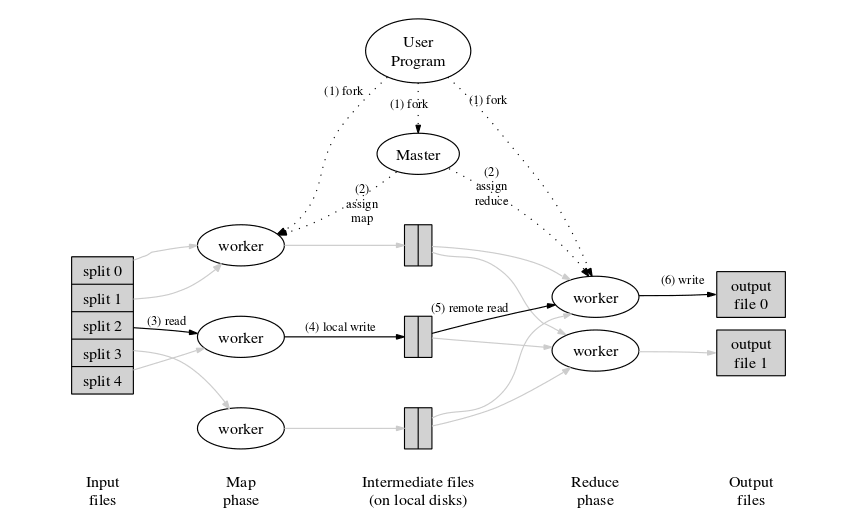
\includegraphics[width=\linewidth]{map-reduce-overview}
  \caption[MapReduce编程模型]{MapReduce编程模型(摘自Google MapReduce论文\cite{Dean2008})}
  \label{fig:map-reduce-overview}
\end{figure}

MapReduce由Google提出\upcite{Dean2008},最初被设计为用于分布式存储计算机集群,
部署在Google的服务器集群之上,执行大规模网络事务处理任务,如网页检索等,表现出很好的性能。
Apache基金会的Hadoop是分布式存储计算机集群上最著名的MapReduce实现。
L\"ammel使用Haskell语言给MapReduce的语义做了精确描述\upcite{Lammel2008}。

Ranger等\upcite{Ranger2007}在共享内存处理器上实现了MapReduce,名为Phoenix,
为MapReduce模型的处理过程提供了更多可配置选项。Phoenix-2是\upcite{Yoo2009}是Phoenix
的改进实现。

MapReduce也被移植到GPU上。香港科技大学的Bingsheng He等在Nvidia GPU上实现了
Mars\upcite{He2008},这是第一个运行在GPU上的Mapreduce系统。由于当时的GPU不支持
动态内存分配,Mars设计了一轮额外的\texttt{map\_count}阶段与一轮额外的\texttt{reduce\_count}
阶段,这带来了一定的附加开销。

MapCG\upcite{Hong2010}是MapReduce系统在GPU上另一版实现。MapCG的贡献是,
统一了MapReduce在CPU端与GPU端的接口设计,并在GPU上实现了一个轻量的动态内存分配器,
从而避免了Mars插入额外处理的开销。

Fang\upcite{Fang2011}增强了了Mars实现,使Mars可以运行在更多并行硬件之上,包括多核CPU、
Nvidia GPU、AMD GPU等,在开发CPU与GPU同时执行计算任务方面进行了一些尝试,
但并未取得理想效果。

Feng\upcite{Ji2011}与Chen\upcite{Chen2012}就GPU片上共享存储器的利用对MapReduce在GPU上
的实现分别提出了不同的优化措施。

Stuart设计了运行在GPU集群上的MapReduce系统GPMR\upcite{Stuart2011}。
出于性能考虑,GPMR向用户暴露了更多硬件细节。GPMR在\texttt{map}阶段
采用了了流水化的执行方式以重叠计算任务与设备间通信。

%% \section{GPU并行编程技术}\label{sec:gpu-parallel-prog}
%% 本节介绍当前使用最广泛的在GPU上进行通用编程的软件技术。

%% \subsection{CUDA}
%% CUDA架构是Nvidia公司针对自己的GPU提出的并行编程框架。
%% 它的提出对GPU通用编程技术产生了巨大的推动力。

%% CUDA为程序员提供了一个完整的GPU编程框架,将GPU的硬件结构
%% 清晰地展现出来。用户使用CUDA C编写在GPU上执行的程序,通常
%% 称为Kernel。CUDA C是一种对C语言的简单扩展,
%% 增加了若干关键字指定程序的执行位置(CPU还是GPU)、变量
%% 的存储位置(全局存储还是贡献存储),
%% 提供了一些内置变量一边获得某些运行时信息。

%% CUDA采用STMD编程模型,这是一种类似与SPMD的编程模型,
%% 一个Kernel程序被一组线程执行,执行路径一般和线程在组中所处的位置相关。
%% 线程按照层次化组织,grid

%% \subsection{OpenCL}

%% \subsection{OpenACC \& OpenHMPP}



%%% Local Variables:
%%% mode: latex
%%% TeX-master: "../main"
%%% End:

\begin{ack}
  衷心感谢导师 xxx 教授和 xxx 副教授对本人的精心指导。他们的言传身教将使我终生受益。

  感谢 \nudtpaper{},它的存在让我的论文写作轻松自在了许多,让我的论文格式规整漂亮了许多。

\end{ack}


%</thesis>
%    \end{macrocode}
%
% 在\LaTeX{}下管理参考文献将极其方便,建议使用Jabref生成条目,
% 用\verb|\cite|(其中\verb|upcite|是上标索引)索引即可。
% \verb|refs.bib|是你的参考文献名。
%    \begin{macrocode}
%<*thesis>
\cleardoublepage
\phantomsection
\addcontentsline{toc}{chapter}{参考文献}
\bibliographystyle{bstutf8}
\bibliography{ref/refs}

\begin{resume}

  \section*{发表的学术论文} % 发表的和录用的合在一起

  \begin{enumerate}[{[}1{]}]
  \addtolength{\itemsep}{-.36\baselineskip}%缩小条目之间的间距,下面类似
  \item Yang Y, Ren T L, Zhang L T, et al. Miniature microphone with silicon-
    based ferroelectric thin films. Integrated Ferroelectrics, 2003,
    52:229-235. (SCI 收录, 检索号:758FZ.)
  \item 杨轶, 张宁欣, 任天令, 等. 硅基铁电微声学器件中薄膜残余应力的研究. 中国机
    械工程, 2005, 16(14):1289-1291. (EI 收录, 检索号:0534931 2907.)
  \item 杨轶, 张宁欣, 任天令, 等. 集成铁电器件中的关键工艺研究. 仪器仪表学报,
    2003, 24(S4):192-193. (EI 源刊.)
  \item Yang Y, Ren T L, Zhu Y P, et al. PMUTs for handwriting recognition. In
    press. (已被 Integrated Ferroelectrics 录用. SCI 源刊.)
  \item Wu X M, Yang Y, Cai J, et al. Measurements of ferroelectric MEMS
    microphones. Integrated Ferroelectrics, 2005, 69:417-429. (SCI 收录, 检索号
    :896KM.)
  \item 贾泽, 杨轶, 陈兢, 等. 用于压电和电容微麦克风的体硅腐蚀相关研究. 压电与声
    光, 2006, 28(1):117-119. (EI 收录, 检索号:06129773469.)
  \item 伍晓明, 杨轶, 张宁欣, 等. 基于MEMS技术的集成铁电硅微麦克风. 中国集成电路, 
    2003, 53:59-61.
  \end{enumerate}

  \section*{研究成果} % 有就写,没有就删除
  \begin{enumerate}[{[}1{]}]
  \addtolength{\itemsep}{-.36\baselineskip}%
  \item 任天令, 杨轶, 朱一平, 等. 硅基铁电微声学传感器畴极化区域控制和电极连接的
    方法: 中国, CN1602118A. (中国专利公开号.)
  \item Ren T L, Yang Y, Zhu Y P, et al. Piezoelectric micro acoustic sensor
    based on ferroelectric materials: USA, No.11/215, 102. (美国发明专利申请号.)
  \end{enumerate}
\end{resume}

%</thesis>
%    \end{macrocode}
%
%<thesis>% 最后,需要的话还要生成附录,全文随之结束。
%    \begin{macrocode}
%<*thesis>
\appendix
\backmatter
\chapter{Rat形式语法}\label{chap:formal-syntax}

\setlength{\grammarindent}{10em}
\setlength{\grammarparsep}{5pt}
\paragraph{Syntax Rules}
\begin{grammar}
<program>        ::=    <export>+ <top level unit>*

<export>         ::=    'export' <variable>

<top level unit> ::=    <type def>
                 \alt     <variable decl>
                 \alt     <variable def>

<type def>       ::=    'newtype' <type name> '=' <constructor> <type spec>

<constructor>    ::=    <variable>

<type spec>      ::=    <primitive type>
                 \alt     <struct type>
                 \alt     <vector type>
                 \alt     <type spec> '$\to$' <type spec>

<primitive type> ::=    'Int8' | 'UInt8' | 'Int16' | 'UInt16' \alt 'Int32' | 'UInt32' | 'Int64' | 'UInt64'
                 \alt     'Float' | 'Double'

<struct type>    ::=    '\{' <variable decl> (',' <variable decl>)* '\}'

<vector type>    ::=    '[' <type name> ']'

<variable decl>  ::=    <variable> '::' <type name>

<variable def>   ::=    <variable> <variable>* '=' <expression>

<expression>     ::=    <literal>
                 \alt     <variable ref>
                 \alt     <function app>
                 \alt     <lambda exp>
                 \alt     <vector comprehension>
                 \alt     <vector element ref>
                 \alt     <vector slice ref>
                 \alt     <conditional>
                 \alt     <let exp>
                 \alt     <where exp>
                 \alt     '(' <expression> ')'

<literal>        ::=    <number>
                 \alt     <boolean>
                 \alt     <character>
                 \alt     <tuple literal>
                 \alt     <vector literal>

<tuple literal>  ::=    '(' <literal> (',' <literal>)+ ')'

<vector literal> ::=    '[' <start> ',' <end> (',' <step>)? ']'

<start>          ::=    <number>

<end>            ::=    <number>

<step>           ::=    <number>

<variable ref>   ::=    <variable>

<function app>   ::=    <function ref> <expression>*

<function ref>   ::=    <variable>

<lambda exp>     ::=    '$\backslash$' <bind var>+ '$\to$' <expression>

<bind var>       ::=    <variable>

<conditional>    ::=    'if' <test> <if clause> <else clause>?

<test>           ::=    <expression>

<if clause>      ::=    <expression>

<else clause>    ::=    <expression>

<vector comprehension>
                 ::=    '[' <expression> \\('|' <generator> (',' (<generator> | <filter>))+ ']'

<generator>      ::=    <variable> '$\gets$' <variable>

<filter>         ::=    <expression>

<vector element ref>
                 ::=    <variable> '[' <index> ']'

<index>          ::=    <expression>

<vector slice ref>
                 ::=    <variable> '[' <index> ':' <index> (',' <index>)? ']'

<let exp>        ::=    'let' <variable decl>+ <variable def>+ 'in' <expression>

<where exp>      ::=    <expression> 'where' <variable decl>+ <variable def>+
\end{grammar}

\paragraph{Lexical Rules}
\begin{grammar}
<variable>       ::=    <lower id> | <special var>

<lower id>       ::=    <lowercase> (<alpha> | <digit> | '\_')*

<special var>    ::=    '+' | '-' | '*' | '/' | '\^'

<class name>     ::=    <upper id>

<type name>      ::=    <upper id>

<upper id>       ::=    <uppercase> (<alpha> | <digit> | '_')*

<alpha>          ::=    <lowercase> | <uppercase>

<lowercase>      ::=    'a' | 'b' | ... | 'z'

<uppercase>      ::=    'A' | 'B' | ... | 'Z'

<number>         ::=    <integer>
                 \alt     <floating>

<integer>        ::=    <decimal>
                 ::=    ('0O' | '0o') <octal>
                 ::=    ('0X' | '0x') <hexadecimal>

<decimal>        ::=    <digit>+

<octal>          ::=    <octit>+

<hexadecimal>    ::=    <hexit>+

<digit>          ::=    '0' | '1' | '2' | '3' | '5' | '6' | '7' | '8' | '9'

<octit>          ::=    '0' | '1' | '2' | '3' | '5' | '6' | '7'

<hexit>          ::=    <digit> | 'A' | 'B' | 'C' | 'D' | 'E' | 'F' | 'a' | 'b' | 'c' | 'd' | 'e' | 'f'

<floating>       ::=    <decimal> '.' <decimal> <exponent>?
                 \alt     <decimal> <exponent>

<exponent>       ::=    ('e' | 'E') ('+' | '-')? <decimal>

<boolean>        ::=    'true' | 'false'

<character>      ::=    ''' <ascii> '''

<whitespace>     ::=    <space> | <tab> | <newline> | <comment>

<comment>        ::=    '--' <any character>* <newline>
\end{grammar}


\end{document}
%</thesis>
%    \end{macrocode}
%
% 当然还有一些收尾工作,校验审阅自不必说。接下来你需要:修改论文中英文日期,
% 生成盲评,生成明(盲)评A3封面。
%
% {\color{blue}Happy \TeX{}ing! 欢迎提各式各样的意见!}
%
% \newpage\relax%
%
% \StopEventually{\PrintChanges}
% \clearpage
%
% \section{实现细节}
% 我们首先介绍文档模板的基本信息以及宏包和配置,
% 然后依照国防科学技术大学论文模板的书写规范一节一节的介绍实现步骤。
%
% \changes{v1.2}{2009/09/28}{添加了A3封面制作}
%
% \subsection{基本信息}
%    \begin{macrocode}
%<cls>\NeedsTeXFormat{LaTeX2e}[1999/12/01]
%<cls>\ProvidesClass{nudtpaper}
%<cfg>\ProvidesFile{nudtpaper.cfg}
%<cls|cfg>[2011/07/17 v2.2 NUDT paper template]
%    \end{macrocode}
%
% \subsection{宏包配置}
%
%<*cls>
%
%\changes{v0.99}{2009/08/17}{add package options}
% 当前的宏包选项在之前已经介绍了,下面是实现步骤,就是几个\verb|if|。
%\changes{v1.6}{2009/12/01}{添加单独的单双面控制}
%\changes{v2.0}{2010/11/09}{添加盲评控制}
%
%    \begin{macrocode}
\newif\ifismaster\ismastertrue
\newif\ifisttf\isttftrue
\DeclareOption{master}{\ismastertrue}
\DeclareOption{doctor}{\ismasterfalse}
\newif\ifisanon\isanonfalse
\DeclareOption{anon}{\isanontrue}
\newif\ifistwoside\istwosidefalse
\DeclareOption{twoside}{\istwosidetrue}
\DeclareOption{ttf}{\isttftrue}
\DeclareOption{otf}{\isttffalse}
\newif\ifisvista\isvistafalse
\DeclareOption{vista}{\isvistatrue}
\DeclareOption*{\PackageWarning{nudtpaper}{Unknown Option '\CurrentOption'}}
\ProcessOptions\relax
%    \end{macrocode}
%
% 首先调用在文档类书写中需要的过程控制语句,在计算一些\verb|length|时要用到
%    \begin{macrocode}
\RequirePackage{ifthen,calc}
%    \end{macrocode}
%
% 接着我们导入文本类,该模板基于标准的书籍模板book,其默认格式为单面打印。
% 博士论文如需双面打印,必须指定\verb|twoside|选项。双开的含义是章节总是
% 起在右手边,左手空白页为完全的空白页,不包含页眉页脚。
%
% \changes{v1.6}{2009/12/01}{修改开关选项}
%
%    \begin{macrocode}
\ifistwoside
  \LoadClass[a4paper,12pt,openright,twoside]{book}
\else
  \LoadClass[a4paper,12pt,openany]{book}
\fi
%    \end{macrocode}
%
% 我们直接用\textsf{geometry}宏包进行页面边距的设定,调用titlesec设定标题以及页眉页脚,
% 用\textsf{titletoc}设定目录格式。需要改动的可以参考这三个宏包的说明文档。
%
%    \begin{macrocode}
\RequirePackage[includeheadfoot]{geometry}
\RequirePackage[center,pagestyles]{titlesec}
\RequirePackage{titletoc}
%    \end{macrocode}
%
% 文档中另外重要的两个部分是表格和图片。
% 首先来看图片:\textsf{graphicx}宏包是必不可少的,
% 并排图形。\textsf{subfigure} 已经不再推荐,用新的 \textsf{subfig}。
% 加入 \verb|config| 选项
% 以便兼容 \textsf{subfigure} 的命令。浮动图形和表格标题样式。\textsf{caption2} 已经不
% 推荐使用,采用新的 \textsf{caption}。它会自动被 \textsf{subfig} 装载进来。所以可以在
% 后面使用 \textbf{captionsetup} 命令,宏包\textsf{float}的作用是可以用H命令,
% 将浮动对象强制放在这里(副作用是版面可能不好):
%
%    \begin{macrocode}
\RequirePackage{graphicx}
\RequirePackage[config]{subfig}
\RequirePackage{float}
%    \end{macrocode}
%
% 再来看表格:我们采用\textsf{longtable}来处理长的表格,还需要\textsf{array}包;
% 标准的论文需要表格为三线表,这里引用\textsf{booktabs}宏包来处理,
% 这样,我们就可以简单的使用\verb|\toprule|,\verb|\midrule|,\verb|bottomrulle|
% 这样的命令;
% 为了在表格中支持跨行,需要引入\textsf{multirow}包,\textsf{tabularx}的作用是为了使用
% 固定宽度的表格,\textsf{slashbox}可以让我们在表格中使用反斜线:
%    \begin{macrocode}
\RequirePackage{array}
\RequirePackage{longtable}
\RequirePackage{booktabs}
\RequirePackage{multirow}
\RequirePackage{tabularx}
\RequirePackage{slashbox}
%    \end{macrocode}
% 表格和图片的例子可以搜索C\TeX{}论坛或者看示例文件。
%
% 引入\textsf{paralist}来达到比较好看的列表环境
%    \begin{macrocode}
\RequirePackage[neverdecrease]{paralist}
%    \end{macrocode}
%
% 文档中还需要一定的色彩控制和字体控制
%    \begin{macrocode}
\RequirePackage{xcolor}
%    \end{macrocode}
%
% 为了排出漂亮的数学公式,\textsf{amsmath}包是必不可少的,
% 需要注意的是,新版本的论文模板仍旧使用\textsf{txfonts}宏包,
% 为了支持希腊正体字母,需要调用\verb|upgreek.sty|,使用方法是\verb|\up<greek>|。
% 注意到这个宏包前面加上了\verb|Symbolsmallscale|选项,这是为了配合
% \verb|txfonts|希腊字体的大小而设定的。如果用户不满意这个宏包的积分号
% 等符号,倾向与使用传统的\LaTeX{}风格的数学符号,那么可以使用
% \textsf{mathptmx}宏包,但要把\verb|upgreek|的选项改为\verb|Symbol|,要不然
% 正体希腊字母要显得小一点哦。
% 而大写斜体希腊字母(变量)可以通过\textsf{amsmath}的\verb|\var<Greek>|得到。
% 当然,对于希腊字母的加粗推荐使用\verb|bm|宏包,一般变量的加粗那就使用
% \verb|\mathbf|吧!
% \changes{v2.0}{2010/11/09}{去掉fontspec,传递no-math到xeCJK,加入bm宏包}
% \changes{v2.2}{2011/07/16}{去掉txfonts宏包,使用lm字体,添加svgreek.sty}
% \changes{v2.2}{2011/07/16}{修改,仍旧使用upgreek, mathptmx, bm组合}
% \changes{v2.2}{2011/09/25}{修改,使用upgreek, txfonts, bm组合}
% \changes{v2.2}{2012/11/28}{给用户提供额外的选项,还是mtpro比较漂亮}
%    \begin{macrocode}
\RequirePackage{amsmath,amssymb}
\RequirePackage{txfonts}
\RequirePackage[Symbolsmallscale]{upgreek}
\RequirePackage{bm}
\RequirePackage[T1]{fontenc}
\RequirePackage[amsmath,thmmarks,hyperref]{ntheorem}
%    \end{macrocode}
% 需要注意的是,如果用户有\verb|mtpro2|包,还是强烈建议使用这个的,因为数学公式
% 在这个包下显得特别的美观。具体在哪里下载或者怎么安装不属于这篇使用说明的范畴。
%
% 本文档类直接采用\XeTeX{}引擎,方便了字体配置以及编译,
% 这里需要调用\textsf{XeCJK}宏包,no--math的作用是不改变先前数学宏包设定的数学字体。
% 同时采用\textsf{indentfirst}宏包管理文字的缩进:
% \changes{v1.8}{2010/10/15}{修改了默认的xeCJK的选项,为了兼容旧的xeCJK版本,normalindentfirst选项暂不使用,而是在后面添加indentfirst包}
% \changes{v2.0}{2010/11/10}{传递no-math给xeCJK里面的fontspec宏包}
% \changes{v2.2}{2011/07/03}{移除CJKtextspace, CJKmathspace, CJKnumber选项}
%
%    \begin{macrocode}
\RequirePackage[CJKnumber,CJKchecksingle,no-math]{xeCJK}
\RequirePackage{indentfirst}
%    \end{macrocode}
%
% 另外一个关键部分是文献索引,包括书签以及参考文献的索引,记得\textsf{hyperref}配合
% \XeTeX{}使用时暂不能开启Unicode选项,新的发行版已经移除\textsf{hypernat}包:
% \changes{v2.1}{2010/12/29}{移除hypernat包}
% \changes{v2.2}{2011/07/17}{移除hyperref的CJKbookmarks旋向}
%    \begin{macrocode}
\RequirePackage[numbers,sort&compress,square]{natbib}
\RequirePackage[pdfborder=0 0 1]{hyperref}
%    \end{macrocode}
%</cls>
%
%\subsection{基础配置}
% 本章主要介绍模板中用到的基本的元素和定义,现在包括两部分: 字体,字号和字体命令
%
%\subsubsection{字体定义}
% 我们首先来处理\TeX{}中最令人棘手的字体问题,
% 在使用\textsf{XeCJK}包之后,配置和选择很容易,
% 预先设定好一些字体命令是为了后面方便的更改文本字体的需要。
% 首先我们开启\TeX{}连字符:
%    \begin{macrocode}
%<*cls>
\defaultfontfeatures{Mapping=tex-text}
%</cls>
%    \end{macrocode}
%
% 之后用\textsc{XeCJK}包提供的命令设定字体,用户可以选择使用TTF还是OTF字体,
% Adobe的OpenType字体在排版上更具备优势,文档显示锐利,推荐使用。
% \verb|setcharclass|的作用是纠正xunicode、xeCJK的一些设定:
%
% \changes{v0.99}{2009/08/17}{add options TTF and OTF}
% \changes{v0.993}{2009/08/25}{加入VISTA用户选项}
% \changes{v1.9}{2010/10/28}{定义一个cusong字体,使用的是中宋}
%
%    \begin{macrocode}
%<*cls>
\xeCJKsetcharclass{"0}{"2E7F}{0}
\xeCJKsetcharclass{"2E80}{"FFFF}{1}
\newcommand\installTTF{%
  \setmainfont{Times New Roman}
  \setsansfont{Arial}
  \setmonofont{Courier New}
  \ifisvista
    \setCJKmainfont[BoldFont={SimHei},ItalicFont={KaiTi}]{SimSun}
    \setCJKmonofont{KaiTi} % Pluto use LiSu Thu use Kaiti, orig is SimSun
    \setCJKfamilyfont{fs}{FangSong}
    \setCJKfamilyfont{kai}{KaiTi}
  \else
    \setCJKmainfont[BoldFont={SimHei},ItalicFont={KaiTi_GB2312}]{SimSun}
    \setCJKmonofont{KaiTi_GB2312} % Pluto use LiSu Thu use Kaiti, orig is SimSun
    \setCJKfamilyfont{fs}{FangSong_GB2312}
    \setCJKfamilyfont{kai}{KaiTi_GB2312}
  \fi
  \setCJKsansfont{SimHei}
  \setCJKfamilyfont{song}{SimSun}
  \setCJKfamilyfont{hei}{SimHei}
  \setCJKfamilyfont{li}{LiSu}
  \setCJKfamilyfont{you}{YouYuan}
}
\newcommand\installOTF{%
  \setmainfont{Times New Roman} % could be changed to "Times New Roman PS Std"
  \setsansfont{Arial}
  \setmonofont{Courier New}
  \setCJKmainfont[BoldFont={Adobe Heiti Std},ItalicFont={Adobe Kaiti Std}]{Adobe Song Std}
  \setCJKsansfont{Adobe Heiti Std}
  \setCJKmonofont{Adobe Kaiti Std}
  \setCJKfamilyfont{song}{Adobe Song Std}
  \setCJKfamilyfont{hei}{Adobe Heiti Std}
  \setCJKfamilyfont{fs}{Adobe Fangsong Std}
  \setCJKfamilyfont{kai}{Adobe Kaiti Std}
  \setCJKfamilyfont{li}{Adobe Kaiti Std}
  \setCJKfamilyfont{you}{Adobe Kaiti Std}
}
\setCJKfamilyfont{cusong}{STZhongsong}
\newcommand{\cusong}{\CJKfamily{cusong}} % 中宋作为加粗宋体
%</cls>
%    \end{macrocode}
%
% \changes{v1.6}{2009/12/01}{替换OTF英文字体为标准Windows自带字体}
% 之后我们根据你的设定决定安装什么字体:
%
%    \begin{macrocode}
%<*cls>
\ifisttf
  \installTTF
\else
  \installOTF
\fi
%</cls>
%    \end{macrocode}
%
% 选定好字体之后,就是设定字体别名,这样我们就可以在文档的其他部分直接使用较短的命令来
% 指定特定的字体了:
%
%    \begin{macrocode}
%<*cls>
\newcommand{\song}{\CJKfamily{song}}    % 宋体
\newcommand{\fs}{\CJKfamily{fs}}        % 仿宋体
\newcommand{\kai}{\CJKfamily{kai}}      % 楷体
\newcommand{\hei}{\CJKfamily{hei}}      % 黑体
\newcommand{\li}{\CJKfamily{li}}        % 隶书
\newcommand{\you}{\CJKfamily{you}}      % 幼圆
\def\songti{\song}
\def\fangsong{\fs}
\def\kaishu{\kai}
\def\heiti{\hei}
\def\lishu{\li}
\def\youyuan{\you}
%</cls>
%    \end{macrocode}
%
% \subsubsection{字号定义}
%下面就是定义字号大小,这一部分我们有两个参考,其一是:
%
% \begin{verbatim}
% 参考科学出版社编写的《著译编辑手册》(1994年)
% 七号      5.25pt       1.845mm
% 六号      7.875pt      2.768mm
% 小五      9pt          3.163mm
% 五号      10.5pt       3.69mm
% 小四      12pt         4.2175mm
% 四号      13.75pt      4.83mm
% 三号      15.75pt      5.53mm
% 二号      21pt         7.38mm
% 一号      27.5pt       9.48mm
% 小初      36pt         12.65mm
% 初号      42pt         14.76mm
%
% 这里的 pt 对应的是 1/72.27 inch,也就是 TeX 中的标准 pt
% \end{verbatim}
%
% 另外一个来自WORD中的设定:
% \begin{verbatim}
% 初号 = 42bp = 14.82mm = 42.1575pt
% 小初 = 36bp = 12.70mm = 36.135 pt
% 一号 = 26bp = 9.17mm = 26.0975pt
% 小一 = 24bp = 8.47mm = 24.09pt
% 二号 = 22bp = 7.76mm = 22.0825pt
% 小二 = 18bp = 6.35mm = 18.0675pt
% 三号 = 16bp = 5.64mm = 16.06pt
% 小三 = 15bp = 5.29mm = 15.05625pt
% 四号 = 14bp = 4.94mm = 14.0525pt
% 小四 = 12bp = 4.23mm = 12.045pt
% 五号 = 10.5bp = 3.70mm = 10.59375pt
% 小五 = 9bp = 3.18mm = 9.03375pt
% 六号 = 7.5bp = 2.56mm
% 小六 = 6.5bp = 2.29mm
% 七号 = 5.5bp = 1.94mm
% 八号 = 5bp = 1.76mm
%
% 1bp = 72.27/72 pt
% \end{verbatim}
%
% 我们采用习惯的字号设定方法(也就是WORD中的设定),首先编写字体设置命令:
%
%\begin{macro}{\choosefont}
% 我们可以使用 |\choosefont| 来选择字体, 字体设定这些大多是从清华的模板拷过来的。
%
%    \begin{macrocode}
%<*cls>
\newlength\thu@linespace
\newcommand{\thu@choosefont}[2]{%
    \setlength{\thu@linespace}{#2*\real{#1}}%
    \fontsize{#2}{\thu@linespace}\selectfont}
\def\thu@define@fontsize#1#2{%
    \expandafter\newcommand\csname #1\endcsname[1][\baselinestretch]{%
    \thu@choosefont{##1}{#2}}}
%</cls>
%    \end{macrocode}
%\end{macro}
%
%设定具体的字体大小:
%
%    \begin{macrocode}
%<*cls>
\thu@define@fontsize{chuhao}{42bp}
\thu@define@fontsize{xiaochu}{36bp}
\thu@define@fontsize{yihao}{26bp}
\thu@define@fontsize{xiaoyi}{24bp}
\thu@define@fontsize{erhao}{22bp}
\thu@define@fontsize{xiaoer}{18bp}
\thu@define@fontsize{sanhao}{16bp}
\thu@define@fontsize{xiaosan}{15bp}
\thu@define@fontsize{sihao}{14bp}
\thu@define@fontsize{banxiaosi}{13bp}
\thu@define@fontsize{xiaosi}{12bp}
\thu@define@fontsize{dawu}{11bp}
\thu@define@fontsize{wuhao}{10.5bp}
\thu@define@fontsize{xiaowu}{9bp}
\thu@define@fontsize{liuhao}{7.5bp}
\thu@define@fontsize{xiaoliu}{6.5bp}
\thu@define@fontsize{qihao}{5.5bp}
\thu@define@fontsize{bahao}{5bp}
%</cls>
%    \end{macrocode}
%
%\subsubsection{自定命令}
% 有一些常量,测试,自定义的命令等都放在这里,待到论文逐渐完善之后再做定夺,
% 当然用户自己的命令也可以在此添加,事实上如果natbib传递的是superscript,
% \verb|cite|命令默认就成了上标了。这里不加入这个选项,而是单独编写一个命令:
%
%    \begin{macrocode}
%<*cls>
\newcommand{\upcite}[1]{\textsuperscript{\cite{#1}}} % 上标形式引用
\newcommand{\china}{中华人民共和国}
\def\nudtpaper{\textsc{Nudt}\textsc{Paper}}
\newcommand{\pozhehao}{\kern0.3ex\rule[0.8ex]{2em}{0.1ex}\kern0.3ex}
%</cls>
%    \end{macrocode}
%
%\subsubsection{中文元素}
%
% 默认的页面元素的英文名,诸如Contents为目录,Abstract为摘要等,
% 我们首先将他们一一中文化:
% \changes{v0.992}{2009/08/19}{修改图表编号格式}
% \changes{v1.3}{2009/10/14}{修改图目录和表目录}
%
%    \begin{macrocode}
%<*cls>
\renewcommand\contentsname{目\hspace{1em}录}
\renewcommand\listfigurename{图\hspace{1em}目\hspace{1em}录}
\renewcommand\listtablename{表\hspace{1em}目\hspace{1em}录}
\newcommand\listequationname{公式索引}
\newcommand\equationname{公式}
\renewcommand\bibname{参考文献}
\renewcommand\indexname{索引}
\renewcommand\figurename{图}
\renewcommand\tablename{表}
\renewcommand\appendixname{附录}
\def\CJK@today{\CJKdigits{\the\year} 年 \CJKnumber{\the\month} 月}
\newcommand\zhtoday{\CJK@today}
\newcommand\entoday{\today{}}
%</cls>
%    \end{macrocode}
%
% 好,下面就开始按照论文模板要求进行排版!
%
%\subsection{编写要求}
% 学校规定,论文需采用白色纸双面打印。
% 学位论文用A4($210mm\times{}297mm$)标准大小的白纸,
% 在打字或印刷时,要求纸的四周留足空白边缘,以便装订、复制和读者批注。
% 每一面的上方(天头)和下方(地角)分别留边25mm,左侧(订口)
% 和右侧(切口)分别留边30mm,页眉与页脚分别为23mm。
%
% 实现起来很简单,只要调用\textsf{geometry}的版面控制命令即可,
% 方法为先把word模板转化为PDF,
% 用Adobe的裁剪功能查看页边距,进行微调,直到比对正确为止,设定如下:
%
% \changes{v0.991}{2009/08/18}{modify bottom skip}
% \changes{v1.1}{2009/09/26}{修改footskip容限以及bottom的值,为了容下longtab的''下一页''}
% \changes{v1.4}{2009/10/28}{减小页眉skip 1mm,用word叠印}
% \changes{v1.4}{2009/10/30}{增大页眉sep .5mm,用word叠印}
%
%    \begin{macrocode}
%<*cls>
\geometry{top=21mm,bottom=25.5mm,left=30mm,right=30mm}
\geometry{headheight=9mm,headsep=1mm,footskip=9mm}
%</cls>
%    \end{macrocode}
%
%\subsection{页眉页脚}
%
% 我们采用titlesec进行页面配置。
% 页面中的主要元素有Chapter,Section,Subsection等元素的外观,
% 位置,颜色字体等,页面元素还包括页眉页脚。这种方法配置简便,易管理。
% 国防科大的论文需要在页眉处画两根横线,我们通过下面的命令实现:
%
%\begin{macro}{\setheadrule}
% 这个命令属于更改\textsf{titlesec}中的一个画页眉的命令,稍加调整:
% \changes{v0.991}{2009/08/18}{modify headrull, s.t. all geometry match}
% \changes{v1.9}{2010/10/28}{去掉headsep,修改headrule,在sethead后添加raisebox}
%
%    \begin{macrocode}
%<*cls>
\renewcommand\setheadrule[1]{%
  \ifdim#1=\z@
    \let\makeheadrule\@empty
  \else
    \def\makeheadrule{%
    \makebox[0pt][l]{\rule[.2\baselineskip]{\linewidth}{1.5pt}}%
    \rule{\linewidth}{1.5pt}}%
  \fi}
%</cls>
%    \end{macrocode}
%\end{macro}
%
% 由于Chapter第一页默认是\verb|plain|页面格式,
% 章节的其余部分是在Matter中设定的页面格式,为了简单起见,
% 我们就直接更改\verb|plain|页面设置,
% 要求为5号宋体居中放置,画页眉页脚,页脚为1磅黑线
%
% \changes{v0.992}{2009/08/20}{renewpagestyle里面前导的空格可能导致clearpage生成新的一页,将空格去掉}
% \changes{v0.993}{2009/08/26}{修改标题,博士硕士对应不同的页眉}
%
%    \begin{macrocode}
%<*cls>
\renewpagestyle{plain}{
\sethead{}{\raisebox{.65\baselineskip}{\songti \wuhao \ifisanon{~}\else{国防科学技术大学研究生院\@optionpaperclass{}学位论文}\fi}}{}%
\setfoot{}{{\songti \wuhao 第~\thepage~页}}{}%
\headrule%
\footrule%
}
\setfootrule{1bp}
%</cls>
%    \end{macrocode}
%
%\subsection{编写格式}
%
% 当页面设置好之后,就是在论文的不同部分分别调用,一般来说论文类的书籍
% 分为三个matter,为前言区(前置部分),正文区(主体),后文区(附录),
% 在国防科大论文书写要求中,
% 需要将摘要单独进行页码编号,其编号为小写罗马字母,为此,
% 可以将摘要单独设定为一个matter,
% 名叫就叫做MidMatter,称作摘要区。每个Matter我们都一一介绍。
%
% 首先看前置部分,主要包括封面,目录,摘要等,实现为:
%
%    \begin{macrocode}
%<*cls>
\renewcommand\frontmatter{%
    \if@openright\cleardoublepage\else\clearpage\fi
    \@mainmatterfalse
    \pagenumbering{Roman}
    \pagestyle{plain}}
\newcommand\midmatter{%
    \if@openright\cleardoublepage\else\clearpage\fi
    \@mainmatterfalse
    \pagenumbering{roman}
    \pagestyle{plain}}
%</cls>
%    \end{macrocode}
%
% 之后为文章的正文区,采用阿拉伯数字编页码:
%
%    \begin{macrocode}
%<*cls>
\renewcommand\mainmatter{%
    \if@openright\cleardoublepage\else\clearpage\fi
    \@mainmattertrue
    \pagenumbering{arabic}
    \pagestyle{plain}}
%</cls>
%    \end{macrocode}
%
% 最后是附录部分,由于他的章节标题与正文中不一样(不是第几章,而是附录几),
% 我们需要单独设定:
%
%    \begin{macrocode}
%<*cls>
\renewcommand\backmatter{%
    \if@openright\cleardoublepage\else\clearpage\fi
    \titleformat{\chapter}{\filcenter \heiti \sanhao}{附录\,\thechapter\,}{1em}{}
    \titlecontents{chapter}[0pt]{\vspace{0.25\baselineskip} \heiti \xiaosi[1.25]}
      {附录\,\thecontentslabel\quad}{}
      {\hspace{.5em}\titlerule*{.}\contentspage}
    \@mainmattertrue
    \pagestyle{plain}}
%</cls>
%    \end{macrocode}
%
% 我们重新定义\verb|cleardoublepage|,使得生成完全的空白页,页面模式为\verb|empty|
%    \begin{macrocode}
%<*cls>
\renewcommand\cleardoublepage{\clearpage\if@openright \ifodd\c@page\else
  \newpage{}
  \thispagestyle{empty}
  \vspace*{\fill}
  \begin{center}
  \end{center}
  \vspace*{\fill}
  \clearpage\fi\fi%
}
%</cls>
%    \end{macrocode}
%
%\subsubsection{前置目录}
% 前置部分的封面在后面详细介绍。首先看目录,要求为:
% 目次页由论文的章、节、条、项、附录等的序号、名称和页码组成,
% 另页排在序之后。目次页标注学位论文的前三级目录。
% 标题统一用“目录”,黑体3字号字居中,段前、段后间距为1行;
% 各章(一级目录)名称用黑体小4号字,段前间距为0.5行,
% 段后间距为0行; 其它(二、三级目录)用宋体小4号字,
% 段前、段后间距为0行。:
%
% 在\LaTeX{}中,Chapter在目录中默认是没有点的,我们加上,另外我们一并将
% 目录中的section和subsection设定好,
% \changes{v0.991}{2009/08/18}{modify TOC baselineskip and font lineskip to 1.25}
%
%    \begin{macrocode}
%<*cls>
\titlecontents{chapter}[0pt]{\vspace{0.25\baselineskip} \heiti \xiaosi[1.25]}
    {第\CJKnumber{\thecontentslabel}章\quad}{}
    {\hspace{.5em}\titlerule*{.}\contentspage}
\titlecontents{section}[2em]{\songti \xiaosi[1.25]}
    {\thecontentslabel\quad}{}
    {\hspace{.5em}\titlerule*{.}\contentspage}
\titlecontents{subsection}[4em]{\songti \xiaosi[1.25]}
    {\thecontentslabel\quad}{}
    {\hspace{.5em}\titlerule*{.}\contentspage}
%</cls>
%    \end{macrocode}
%
% 然后是表目录和图目录,内容用宋体小4号字,在同学使用模板时,需要标题对齐,
% 我们一并在这里实现:
% \changes{v0.993}{2009/08/25}{添加makebox使得图表标题对齐}
%
%    \begin{macrocode}
%<*cls>
\titlecontents{figure}[0pt]{\songti \xiaosi[1.25]}
    {\makebox[3.5em][l]{图~\thecontentslabel\quad}}{}
    {\hspace{.5em}\titlerule*{.}\contentspage}
\titlecontents{table}[0pt]{\songti \xiaosi[1.25]}
    {\makebox[3.5em][l]{表~\thecontentslabel\quad}}{}
    {\hspace{.5em}\titlerule*{.}\contentspage}
%</cls>
%    \end{macrocode}
%
% 书籍模板中,在LOF或者LOT章节之间会默认插入额外的距离,我们通过修改下面这个命令移除,
% 这个方法不是一个完美的办法,\textbf{注意}:下面的代码不要去深究或者理解,
% 这只是把book.cls中的内容复制过来,然后去掉包含addvspace命令的两行。
% 我实在找不出更加好的办法,如果你有,可以联系我。
%
% \changes{v0.993}{2009/08/25}{移除LOF及LOT中章节之间额外的距离}
%
%    \begin{macrocode}
%<*cls>
\renewcommand\chapter{\if@openright\cleardoublepage\else\clearpage\fi
                    \thispagestyle{plain}%
                    \global\@topnum\z@
                    \@afterindentfalse
                    \secdef\nudt@chapter\@schapter}
\def\nudt@chapter[#1]#2{
  \ifnum \c@secnumdepth >\m@ne
    \if@openright\cleardoublepage\else\clearpage\fi
    \phantomsection
    \if@mainmatter
      \refstepcounter{chapter}%
      \addcontentsline{toc}{chapter}%
        {\protect\numberline{\thechapter}#1}%
    \else
      \addcontentsline{toc}{chapter}{#1}%
    \fi
  \else
    \addcontentsline{toc}{chapter}{#1}%
  \fi
  \chaptermark{#1}%
  \if@twocolumn
    \@topnewpage[\@makechapterhead{#2}]%
  \else
    \@makechapterhead{#2}%
    \@afterheading
  \fi
}
%</cls>
%    \end{macrocode}
%
%\subsubsection{前置摘要}
%
% 摘要的要求为题目黑体3字号字居中,段前、段后间距为1行,内容用宋体小4号字,
% 英文摘要内容用Time New Roman小4号字。
% 中文关键字以黑体小4号字另起一行,排在摘要的下方,英文关键字用Arial小4号字。
%
% \changes{v1.8}{2010/10/15}{ABSTRACT和英文关键字需要用Arial字体}
%    \begin{macrocode}
%<*cls>
\newcommand\cabstractname{摘\hspace{1em}要}
\newcommand\eabstractname{ABSTRACT}
\newcommand\ckeywordsname{关键词}
\newcommand\ckeywords[1]{{\hei\xiaosi \ckeywordsname: #1}}
\newcommand\ekeywordsname{Key Words}
\newcommand\ekeywords[1]{\textsf{\xiaosi \ekeywordsname: #1}}
\newenvironment{cabstract}{%
    \chapter{\cabstractname}
    \xiaosi
    \@afterheading}
    {\par\vspace{2em}\par}
\newenvironment{eabstract}{%
    \chapter{\textsf{\eabstractname}}
    \xiaosi
    \@afterheading}
    {\par\vspace{2em}\par}
%</cls>
%    \end{macrocode}
%
%\subsection{主体部分}
%
% \subsubsection{标题格式}
% 要求为:
% \begin{compactenum}
% \item	一级标题(章)用黑体3号字居中,1.25倍行距,段前、段后间距为1行,每一章从新的一页开始;
% \item	二级标题(节)用宋体4号粗体字居中,1.25倍行距,段前、段后间距为1行;
% \item	三级标题用黑体小4号字两端对齐,1.25倍行距,段前、段后间距为1行;
% \item	四级标题用宋体小4号粗体字两端对齐,1.25倍行距,段前间距为0.5行,段后间距为0行;
% \end{compactenum}
%
% \changes{v0.991}{2009/08/18}{按照要求设定标题}
% \changes{v0.992}{2009/08/19}{修改secnumdepth使得subsubsection可用}
% \changes{v1.1}{2009/09/26}{修改Title的spacing为弹性值}
% \changes{v1.2}{2009/10/06}{去掉弹性值,不去生成大量的空白}
% \changes{v1.4}{2009/10/28}{修改chapter段后行距为2ex,段前-1ex,保证上下对称}
% \changes{v1.4}{2009/10/29}{修改chapter段后行距为2.4ex,段前-1.2ex,保证上下对称}
%
% 当章节标题出现的新的一页时,会出现段前距过小的情况,按照milksea的说法是:
% 一般而言,当一个内容在一页开头时,前面的\verb|\vskip|不起作用;
% 类似地,一行开头\verb|\hskip|不起作用。这不是 BUG,如果需要总起效果的间距,
% 用\verb|\vspace*|,文档里面有这样的例子。参照titlesec的文档,需加上:
% \changes{v1.9}{2010/10/28}{增加sectionbreak,设定topskip为0pt}
%
%    \begin{macrocode}
%<*cls>
\newcommand{\sectionbreak}{%
\addpenalty{-300}%
\vspace*{0pt}%
}
\setlength{\topskip}{0pt}
%</cls>
%    \end{macrocode}
% \changes{v1.9}{2010/10/28}{在定义了粗宋字体之后,按照学位论文要求设定标题字体}
% \changes{v1.9}{2010/10/28}{使用了ttltips.pdf的设置chapter距顶端距离的办法}
%
%    \begin{macrocode}
%<*cls>
\setcounter{secnumdepth}{3}
\titleformat{\chapter}{\filcenter \heiti\sanhao[1.25]}{第\CJKnumber{\thechapter}章\,}{1em}{}
\titleformat{\section}{\filcenter \cusong\sihao[1.25]}{\thesection}{1em}{}
\titleformat{\subsection}{\heiti\xiaosi[1.25]}{\thesubsection}{1em}{}
\titleformat{\subsubsection}{\cusong\xiaosi[1.25]}{\thesubsubsection}{1em}{}
\titlespacing{\chapter}{0pt}{2.4ex-\topskip-\heightof{A}}{2.4ex \@plus 2bp \@minus 2bp}
\titlespacing{\section}{0pt}{2ex-\heightof{a}}{2ex \@plus 2bp \@minus 2bp}
\titlespacing{\subsection}{2em}{2ex \@plus 2bp \@minus 2bp}{2ex \@plus 2bp \@minus 2bp}
\titlespacing{\subsubsection}{2em}{1ex \@plus 2bp \@minus 2bp}{0ex \@plus 2bp \@minus 2bp}
%</cls>
%    \end{macrocode}
%
%\subsubsection{正文字体}
% 首先确定正文中使用的字体,文档要求正文字体为小四,行距为固定值1.25倍,
% 中文字体为宋体,英文为{Times New Roman}
%
%\begin{macro}{\normalsize}
% 我们重新定义 |\normalsize| 来确定文档的正文字体,
% 同时修改正文中公式与文字间的距离:
% \changes{v1.9}{2010/10/28}{在normalsize后面每一行加上\%号来吃掉多余的空格}
% \changes{v2.2}{2011/07/16}{减小公式之间距离rubber space的上界}
% \changes{v2.2}{2011/09/25}{减小公式之间距离rubber space的下界}
%
%    \begin{macrocode}
%<*cls>
\renewcommand\normalsize{%
\@setfontsize\normalsize{12bp}{12.87bp}%
\renewcommand{\baselinestretch}{1.3}%
\setlength\abovedisplayskip{10bp \@plus 1bp \@minus 1bp}%
\setlength\abovedisplayshortskip{10bp \@plus 1bp \@minus 1bp}%
\setlength\belowdisplayskip{\abovedisplayskip}%
\setlength\belowdisplayshortskip{\abovedisplayshortskip}%
}
%</cls>
%    \end{macrocode}
%\end{macro}
%
% \changes{v0.991}{2009/08/18}{modify normalsize, which will cause headrule shift}
% \changes{v0.991}{2009/08/18}{add comment on displayskip}
% \changes{v1.0}{2009/09/22}{modify display skip}
%
%\subsubsection{正文段落}
% 接下来还有一个细节就是处理段落缩进,文档设定为首行缩进2个字符,
% 这一个命令需要在文档开始时自动执行:
%
% \changes{v1.3}{2009/10/03}{添加checkparameter这一选项,避免由于更新模板导致未定义的情况出现}
% \changes{v1.7}{2010/04/30}{应当在封面制作完后替换tabular}
%
%    \begin{macrocode}
%<*cls>
\newlength\CJK@twochars
\def\CJK@spaceChar{\Unicode{48}{7}}
\def\CJKindent{%
  \settowidth\CJK@twochars{中国}%
  \parindent\CJK@twochars}
\AtBeginDocument{%
  \CJKindent\relax
  \checkparameter\relax
}
%</cls>
%    \end{macrocode}
%
% 之后定义段落间距,段前间距以及段后间距都为0
% \changes{v0.993}{2009/08/27}{修改parskip}
% \changes{v2.2}{2011/09/25}{修改parskip,允许少量的调整,1bp}
% \changes{v2.2}{2011/10/14}{修改parskip,仅允许负的少量调整,2bp}
%
%    \begin{macrocode}
%<*cls>
\setlength{\parskip}{0bp \@plus 2bp \@minus 2bp}
%</cls>
%    \end{macrocode}
%
% 有时候我们需要手动设定字体间距,该命令在声明页使用过:
%\begin{macro}{\ziju}
%    \begin{macrocode}
%<*cls>
\newcommand*{\ziju}[1]{\renewcommand{\CJKglue}{\hskip #1}}
%</cls>
%    \end{macrocode}
%\end{macro}
%
% \changes{v1.4}{2009/10/26}{推荐用户使用紧凑的列表环境}
%
% 这一部分来自Thuthesis的代码,其出发点是不满意\LaTeX{}默认列表环境间距过大,用
% paralist包中的相关环境进行替代。请参考paralist宏包。
%
% \changes{v1.4}{2009/10/26}{修改参考文献的行距设定}
%
% 而同样有间距问题的是参考文献,两个条目之间过大的距离不是很美观,
% 最简单的办法是修改bibsep变量,如果还是不行,我们直接从thuthesis中拿来代码:
%
% \changes{v1.4}{2009/10/26}{修改参考文献的行距}
% \changes{v1.4}{2009/10/29}{修改参考文献左对齐}
% \changes{v2.2}{2011/10/14}{减小文献列表间距,将penalty改为4000}
%
%    \begin{macrocode}
%<*cls>
\renewenvironment{thebibliography}[1]{%
   \chapter*{\bibname}%
   \list{\@biblabel{\@arabic\c@enumiv}}%
        {\renewcommand{\makelabel}[1]{##1\hfill}
         \settowidth\labelwidth{1.1cm}
         \setlength{\labelsep}{0.4em}
         \setlength{\itemindent}{0pt}
         \setlength{\leftmargin}{\labelwidth+\labelsep}
         \addtolength{\itemsep}{-0.7em}
         \usecounter{enumiv}%
         \let\p@enumiv\@empty
         \renewcommand\theenumiv{\@arabic\c@enumiv}}%
    \sloppy\frenchspacing
    \clubpenalty4000%
    \widowpenalty4000%
    \interlinepenalty4000%
    \sfcode`\.\@m}
   {\def\@noitemerr
     {\@latex@warning{Empty `thebibliography' environment}}%
    \endlist\frenchspacing}
%</cls>
%    \end{macrocode}
%
%\subsection{浮动对象}
%
% 浮动对象针对的目标是图片表格,标题为五号字体,
% 图片标题在下,表格标题在上,具体实现为:
% \changes{v1.1}{2009/09/26}{修改float浮动弹性}
% \changes{v2.2}{2011/09/25}{去掉1.0fil改为4bp, 这样不至于生成过大的空白.}
%
%    \begin{macrocode}
%<*cls>
\setlength{\floatsep}{12bp \@plus 2bp \@minus 2bp}
\setlength{\intextsep}{12bp \@plus 2bp \@minus 2bp}
\setlength{\textfloatsep}{12bp \@plus 2bp \@minus 2bp}
\setlength{\@fptop}{0bp \@plus4bp}
\setlength{\@fpsep}{12bp \@plus4bp}
\setlength{\@fpbot}{0bp \@plus4bp}
%</cls>
%    \end{macrocode}
%
% 接下来设置每一页图形占据的比例,这个直接从\thuthesis{}中拿出,
% 具体含义可以参考下面这个网页:
% \url{http://www.ctex.org/documents/latex/graphics/node69.html},
% 里面解释的很清楚,这个布置方法也是网站的推荐:
% \changes{v1.3}{2009/09/29}{调整floatpagefraction的大小}
% \changes{v2.2}{2011/09/10}{重新调整floatpagefraction,使得更为宽松}
% \changes{v2.2}{2011/09/25}{更为宽松的布置条件}
% \changes{v2.2}{2011/09/25}{更为宽松的布置条件,仿照AMSMATH}
%
%    \begin{macrocode}
%<*cls>
\renewcommand{\textfraction}{0.01}
\renewcommand{\topfraction}{0.99}
\renewcommand{\bottomfraction}{0.99}
\renewcommand{\floatpagefraction}{0.90}
\clubpenalty            =   10000
\widowpenalty           =   10000
\displaywidowpenalty    =   10000
%</cls>
%    \end{macrocode}
%
% 在修改图片标题距离时,要注意,aboveskip为内距离,也就是标题与浮动体之间的距离,
% belowskip为外距离,也就是标题与正文之间的距离。
% \changes{v1.3}{2009/09/29}{缩小图片标题与下文的距离}
% \changes{v1.7}{2010/04/30}{增添LT array命令,可修改Longtable字体大小}
%
%    \begin{macrocode}
%<*cls>
\let\old@tabular\@tabular
\def\thu@tabular{\wuhao[1.25]\old@tabular}
\DeclareCaptionLabelFormat{thu}{{\wuhao[1.25]\song #1~\rmfamily #2}}
\DeclareCaptionLabelSeparator{thu}{\hspace{1em}}
\DeclareCaptionFont{thu}{\wuhao[1.25]}
\captionsetup{labelformat=thu,labelsep=thu,font=thu}
\captionsetup[table]{position=top,belowskip=0bp \@plus 2bp \@minus 2bp,aboveskip=6bp \@plus 2bp \@minus 2bp}%
\captionsetup[figure]{position=bottom,belowskip=-3bp \@plus 2bp \@minus 2bp,aboveskip=6bp \@plus 2bp \@minus 2bp}%
\captionsetup[subfloat]
{labelformat=simple,font=thu,captionskip=6bp,nearskip=6bp,farskip=0bp,topadjust=0bp}
\renewcommand{\thesubfigure}{(\alph{subfigure})}
\renewcommand{\thesubtable}{(\alph{subtable})}
\let\thu@LT@array\LT@array
\def\LT@array{\thu@LT@array}
%</cls>
%    \end{macrocode}
%
%\subsection{自定环境}
%
% 在这里我们自定义一些论文种会使用到的环境,主要有摘要,符号表,致谢,个人介绍等:
% 这些单独定义的环境可以分别配置以满足要求。
%
% 有些论文需要在正文前面加入符号列表, 其内容格式是简单的列表环境:
% \changes{v2.2}{2011/09/10}{略微减小列表间距,与行距相等}
% \changes{v2.2}{2011/09/13}{略微减小标签和说明间距}
%
%    \begin{macrocode}
%<*cls>
\newenvironment{denotation}[1][2.5cm]{
    \chapter*{符号列表} % no tocline
    \noindent\begin{list}{}%
    {\vskip-30bp\xiaosi[1.5]
    \renewcommand\makelabel[1]{##1\hfil}
    \setlength{\labelwidth}{#1} % 标签盒子宽度
    \setlength{\labelsep}{0.75cm} % 标签与列表文本距离
    \setlength{\itemindent}{0cm} % 标签缩进量
    \setlength{\leftmargin}{\labelwidth+\labelsep} % 左边界
    \setlength{\rightmargin}{0cm}
    \setlength{\parsep}{0cm} % 段落间距
    \setlength{\itemsep}{0cm} % 标签间距
    \setlength{\listparindent}{0cm} % 段落缩进量
    \setlength{\topsep}{0pt} % 标签与上文的间距
}}{\end{list}}
%</cls>
%    \end{macrocode}
%
% 致谢往往在正文的最后:
%
% \changes{v1.8}{2010/10/15}{致谢之间要加一个空格}
%    \begin{macrocode}
%<*cls>
\newenvironment{ack}{%
    \chapter*{致\hspace{1em}谢}%
    \addcontentsline{toc}{chapter}{致谢}%
    \ifisanon\color{white}\else\relax\fi%
    \xiaosi%
    \@afterheading}
    {\par\vspace{2em}\par}
%</cls>
%    \end{macrocode}
%
% 个人简历这一部分用来放置作者在研究生期间取得的成果,发表的论文等。可以
% 详细的参考\verb|data/|中的文件自己书写。
% \changes{v1.4}{2009/10/26}{修改标题}
%
%    \begin{macrocode}
%<*cls>
\newenvironment{resume}{%
    \chapter*{作者在学期间取得的学术成果}
    \addcontentsline{toc}{chapter}{作者在学期间取得的学术成果}
    \xiaosi
    \@afterheading}
    {\par\vspace{2em}\par}
%</cls>
%    \end{macrocode}
%
%\subsubsection{定理环境}
% 定理环境可能数学论文中应用较多:
% \changes{v2.0}{2010/11/09}{修改定理的分隔符和QED符号,修改字体;缩进为段落缩进;修改编号}
% \changes{v2.2}{2011/10/14}{设定定理、定义环境的合理间隔}
%
%    \begin{macrocode}
%<*cls>
\renewtheoremstyle{nonumberplain}%
{\item[\hspace*{2em} \theorem@headerfont ##1\ \theorem@separator]}%
{\item[\hspace*{2em} \theorem@headerfont ##1\ (##3)\theorem@separator]}
\theoremstyle{nonumberplain}
\theorembodyfont{\kai\xiaosi[1.3]}
\theoremheaderfont{\hei\xiaosi[1.3]}
\theoremsymbol{\ensuremath{\blacksquare}}
\theoremseparator{:\,}
\newtheorem{proof}{证明}[chapter]
\newtheorem{assumption}{假设}[chapter]
\newtheorem{definition}{定义}[chapter]

\renewtheoremstyle{plain}%
{\item[\hspace*{2em} \theorem@headerfont ##1\ ##2\theorem@separator]}%
{\item[\hspace*{2em} \theorem@headerfont ##1\ ##2\ (##3)\theorem@separator]}
\theoremstyle{plain}
\theorembodyfont{\kai\xiaosi[1.3]}
\theoremheaderfont{\hei\xiaosi[1.3]}
\theoremsymbol{}
\newtheorem{lemma}{引理}[chapter]
\newtheorem{theorem}{定理}[chapter]
\newtheorem{axiom}{公理}[chapter]
\newtheorem{corollary}{推论}[chapter]
\newtheorem{conjecture}{猜想}[chapter]
\newtheorem{proposition}{命题}[chapter]
\newtheorem{exercise}{练习}[section]
\newtheorem{example}{例}[section]
\newtheorem{problem}{问题}[section]
\newtheorem{remark}{注释}[section]
%</cls>
%    \end{macrocode}
%
%\subsection{论文属性}
% 这里的内容主要用来定义封面中的一些元素,你可以像填空一样完成封面的制作:
% \changes{v0.993}{2009/08/26}{添加cosupervisor,协助指导导师}
% \changes{v1.3}{2009/10/03}{添加英文第二导师,增加判断语句,在文档开始时执行}
%
%    \begin{macrocode}
%<*cls>
\def\classification#1{\def\@classification{#1}} % 中图分类号
\def\serialno#1{\def\@serialno{#1}} % 学号
\def\UDC#1{\def\@UDC{#1}} % UDC号
\def\confidentiality#1{\def\@confidentiality{#1}} % 密级
\def\title#1{\def\@title{#1}} % 中文题目
\newtoks\displaytitle
\def\author#1{\def\@author{#1}}
\def\zhdate#1{\def\@zhdate{#1}}	% 中文日期
\def\subject#1{\def\@subject{#1}} % 中文学科
\def\researchfield#1{\def\@researchfield{#1}} % 中文研究方向
\def\supervisor#1{\def\@supervisor{#1}} % 导师
\def\cosupervisor#1{\def\@cosupervisor{#1}} % 协助指导教师
\def\papertype#1{\def\@papertype{#1}} % 工学,理学,同等学历申请工(理)学
\def\entitle#1{\def\@entitle{#1}}
\def\enauthor#1{\def\@enauthor{#1}}
\def\ensupervisor#1{\def\@ensupervisor{#1}}
\def\encosupervisor#1{\def\@encosupervisor{#1}}
\def\endate#1{\def\@endate{#1}}
\def\ensubject#1{\def\@ensubject{#1}}
\def\enpapertype#1{\def\@enpapertype{#1}} % Engineering, Science
\def\optionpaperclass#1{\def\@optionpaperclass{#1}} % paperclass
\def\optionpaperclassen#1{\def\@optionpaperclassen{#1}}
\def\optionas#1{\def\@optionas{#1}} % Advisor OR Supervisor
%</cls>
%    \end{macrocode}
%
% 我们看用户是想用博士封面还是硕士封面:
%
%    \begin{macrocode}
%<*cls>
\ifismaster
  \optionpaperclass{硕士}
  \optionpaperclassen{Master}
  \optionas{Advisor}
\else
  \optionpaperclass{博士}
  \optionpaperclassen{Doctor}
  \optionas{Supervisor}
\fi
%</cls>
%    \end{macrocode}
%
%\subsection{制作封面}
%
% 由于封面中一些元素是可选的,如果在正文中没有定义,那么判断ifx的时候就会出错,
% 我们加入下面的命令进行判断,如果没定义,我们就令他为空。
% 这个命令将在文档开始时自动执行。
%
%    \begin{macrocode}
%<*cls>
\newcommand{\checkparameter}
{
  \ifthenelse{\isundefined{\@cosupervisor}}{\cosupervisor{}}{}
  \ifthenelse{\isundefined{\@encosupervisor}}{\encosupervisor{}}{}
}
%</cls>
%    \end{macrocode}
%
% 制作封面比较复杂,需要一些手动调整的东西,首先来看第一页,
% 重新定义了\verb|maketitle|,
% 用表格来安排页面元素,页头采用仿宋五号字体,段前段后间距一行,这个空一行就用3ex实现,
% \changes{v1.5}{2009/11/18}{微调封面布局}
% \changes{v2.0}{2010/11/09}{标题用粗宋}
% \changes{v2.0}{2010/11/09}{增加盲评控制}
% \changes{v2.1}{2010/11/23}{设定页码为alph,增加cleardoublepage,这样在博士双面时方便打印}
%    \begin{macrocode}
%<*cls>
\def\maketitle{%
  \def\entry##1##2##3{%
    \multicolumn{##1}{l}{\underline{\hbox to ##2{\hfil##3\hfil}}}
    }
  \null
  \ifisanon%
  \author{}%
  \enauthor{}%
  \supervisor{}%
  \cosupervisor{}%
  \ensupervisor{}%
  \encosupervisor{}%
  \else\relax\fi%
  \pagenumbering{alph}% not display, for print only
  \thispagestyle{empty}%
  \begin{center}\leavevmode	% 表格环境
  {\fangsong \wuhao[1.25]%
    \begin{tabular}{llcll}
    分类号 	& \entry{1}{3.2cm}{\@classification} & \hspace*{4.8cm}%
    学号   	& \entry{1}{3.2cm}{\@serialno}         \\[5mm]    %
    U\ D\ C	& \entry{1}{3.2cm}{\@UDC} &            \hspace*{4.8cm}
    密级	& \entry{1}{3.2cm}{\@confidentiality}
    \end{tabular}
  }
  \par
  \vspace*{2.5cm} %插入空白
  {\heiti\sanhao \@papertype{}\@optionpaperclass{}学位论文}\\
  \vspace{12bp}
  {\cusong\erhao[1.25] \@title \par}%
  \vspace{45bp} %从WORD中得来
  {\heiti \sihao
    \begin{tabular}{cp{8cm}c}
      \raisebox{-3.7ex}[0pt]{\@optionpaperclass{}生姓名} &
        {\fs \hfil\raisebox{-3.7ex}[0pt]{\@author}\hfil{}} & \\[3.2ex]
        \cline{2-2}
      \raisebox{-3.7ex}[0pt]{学\ 科\ 专\ 业} &
        {\fs \hfil\raisebox{-3.7ex}[0pt]{\@subject}\hfil{}} & \\[3.2ex]
        \cline{2-2}
      \raisebox{-3.7ex}[0pt]{研\ 究\ 方\ 向} &
        {\fs \hfil\raisebox{-3.7ex}[0pt]{\@researchfield}\hfil{}} & \\[3.2ex]
        \cline{2-2}
      \raisebox{-3.7ex}[0pt]{指\ 导\ 教\ 师} &
        {\fs \hfil\raisebox{-3.7ex}[0pt]{\@supervisor}\hfil{}} & \\[3.2ex]
        \cline{2-2}
      \ifx\@cosupervisor\@empty\else
        & {\fs \hfil\raisebox{-3.7ex}[0pt]{\@cosupervisor}\hfil{}} & \\[3.2ex]
        \cline{2-2}
      \fi
    \end{tabular}
  }
  \end{center}%

  \par
  \vfill
  {\centering \cusong \sanhao \ifisanon{~}\else{国防科学技术大学研究生院}\fi\\[0.8em]
    {\@zhdate \par}%
  }
  \vspace{1mm}
%</cls>
%    \end{macrocode}
%
%第二页主要是论文的英文信息,简称英文封面
%
%    \begin{macrocode}
%<*cls>
  \cleardoublepage%
  \newpage
  \thispagestyle{empty}%

  \begin{center}\leavevmode
  \vfill\bfseries
  {\erhao[1.25] \@entitle \par}
  {\sanhao[1.25]
  \vfill\vfill\vfill\vfill\vfill\vfill
  \begin{tabular}{rl}
    Candidate:\ & {\textsf{\@enauthor}}\\
    \@optionas{}:\ & {\textsf{\@ensupervisor}}\\
    \ifx\@encosupervisor\@empty\else
      & {\textsf{\@encosupervisor}} \\
    \fi
  \end{tabular}}
  \vfill\vfill\vfill\vfill
  {\sanhao[1.5]
A dissertation\\
Submitted in partial fulfillment of the requirements\\
for the degree of \textsf{\@optionpaperclassen{} of \@enpapertype}\\
in \textsf{\@ensubject}\\
\makebox[\textwidth]{\ifisanon{~}\else{Graduate School of National University of %
Defense Technology}\fi}\\
\ifisanon{~}\else{Changsha, Hunan, P.\ R.\ China}\fi\\[5mm]
~\@endate~
  }
  \end{center}\vfill
  \cleardoublepage%
%</cls>
%    \end{macrocode}
%
% 第三页放置独创性声明,这里要使用\verb|displaytitle|这个论文元素:
% \changes{v2.1}{2010/12/29}{表格字体定为五号}
%    \begin{macrocode}
%<*cls>
  \newpage
  \thispagestyle{empty}

  {\cusong \erhao \centering \ziju{12pt} 独创性声明 \par\vspace{2cm}}
    \renewcommand{\baselinestretch}{1.5}%
  {\fangsong\xiaosi %
本人声明所呈交的学位论文是我本人在导师指导下进行的研究工
作及取得的研究成果。尽我所知,除文中特别加以标注和致谢的地方外,论文中
不包含其他人已经发表和撰写过的研究成果,也不包含为获得国防科学技术大学或
其他教育机构的学位或证书而使用过的材料。与我一同工作的同志对本研究所做的
任何贡献均已在论文中作了明确的说明并表示谢意。\par
学位论文题目:\vbox{\hbox to11cm{\hfil \the\displaytitle \hfil}
  \protect\vspace{0.6truemm}\relax
  \hrule depth0pt height0.15truemm width11cm}\par
学位论文作者签名:\hrulefill\hrulefill\hrulefill\hrulefill\hrulefill
  \hfill 日期:\hfill\hfill 年\hfill 月 \hfill 日\hspace{1cm}\par}

  \vspace*{2cm}
  {\cusong \erhao \centering 学位论文版权使用授权书\par\vspace{2cm}}
  {\fangsong\xiaosi %
本人完全了解国防科学技术大学有关保留、使用学位论文的规定。
本人授权国防科学技术大学可以保留并向国家有关部门或机构送交论文的复印件和电子
文档,允许论文被查阅和借阅; 可以将学位论文的全部或部分内容编入有关数据库
进行检索,可以采用影印、缩印或扫描等复制手段保存、汇编学位论文。\par
(保密学位论文在解密后适用本授权书。)\par
学位论文题目:\vbox{\hbox to11cm{\hfil \the\displaytitle \hfil}
  \protect\vspace{0.6truemm}\relax
  \hrule depth0pt height0.15truemm width11cm}\par
学位论文作者签名:\hrulefill\hrulefill\hrulefill\hrulefill\hrulefill
  \hfill 日期:\hfill\hfill 年\hfill 月 \hfill 日\par
作者指导教师签名:\hrulefill\hrulefill\hrulefill\hrulefill\hrulefill
  \hfill 日期:\hfill\hfill 年\hfill 月 \hfill 日\par}

  \normalsize % normal, 正文开始
  \def\@tabular{\wuhao[1.25]\old@tabular} % 之后表格字体使用5号
  \cleardoublepage%
  \newpage
  \thispagestyle{empty}

} % QED
%</cls>
%    \end{macrocode}
%
% \Finale
%
% \iffalse meta-comment
% 下面的配置为本文档使用的模板
% \fi
%
% \iffalse
% \changes{v1.8}{2010/10/15}{按照milksea的说法,修改xltxtra和xunicode相对于xeCJK的顺序}
% \changes{v1.8}{2010/10/15}{添加了xeCJKsetcharclass,使itemize环境正确}
%<*nudtx>
%    \begin{macrocode}
%    \end{macrocode}
%</nudtx>
% \fi
%
\endinput
